% \iffalse meta-comment
%
% Copyright (C) \the\year by Liu Benyuan <liubenyuan@gmail.com>
% This file may be distributed and/or modified under the
% conditions of the LaTeX Project Public License, either
% version 1.2 of this license or (at your option) any later
% version. The latest version of this license is in:
%
% http://www.latex-project.org/lppl.txt
%
% and version 1.2 or later is part of all distributions of
% LaTeX version 1999/12/01 or later.
%
% \fi
% 
% \iffalse
% <package>\NeedsTeXFormat{LaTeX2e}[1999/12/01]
% <package>\ProvidesPackage{nudtpaper}
% <package>		[2009/08/12 v1.0 By Liu Benyuan <liubenyuan@gmail.com>]
%<*driver>
\ProvidesFile{nudtpaper.dtx}[2009/08/12 v1.0 NUDT]
\documentclass[11pt]{ltxdoc}
\usepackage{nudtx}
\EnableCrossrefs
\CodelineIndex
\RecordChanges
\begin{document}
  \DocInput{\jobname.dtx}
\end{document}
%</driver>
% \fi
% 
% \def\thuthesis{\textsc{Thu}\-\textsc{Thesis}}
% \def\nudtpaper{\textsc{Nudt}\-\textsc{Paper}}
% 
% \CheckSum{1224}
% \CharacterTable
%  {Upper-case    \A\B\C\D\E\F\G\H\I\J\K\L\M\N\O\P\Q\R\S\T\U\V\W\X\Y\Z
%   Lower-case    \a\b\c\d\e\f\g\h\i\j\k\l\m\n\o\p\q\r\s\t\u\v\w\x\y\z
%   Digits        \0\1\2\3\4\5\6\7\8\9
%   Exclamation   \!     Double quote  \"     Hash (number) \#
%   Dollar        \$     Percent       \%     Ampersand     \&
%   Acute accent  \'     Left paren    \(     Right paren   \)
%   Asterisk      \*     Plus          \+     Comma         \,
%   Minus         \-     Point         \.     Solidus       \/
%   Colon         \:     Semicolon     \;     Less than     \<
%   Equals        \=     Greater than  \>     Question mark \?
%   Commercial at \@     Left bracket  \[     Backslash     \\
%   Right bracket \]     Circumflex    \^     Underscore    \_
%   Grave accent  \`     Left brace    \{     Vertical bar  \|
%   Right brace   \}     Tilde         \~}
%
% \changes{v0.99}{2009/08/12}{Initial Release}
%
% \GetFileInfo{\jobname.dtx}
% 
% \DoNotIndex{\begin,\end,\begingroup,\endgroup}
% \DoNotIndex{\ifx,\ifdim,\ifnum,\ifcase,\else,\or,\fi}
% \DoNotIndex{\let,\def,\xdef,\newcommand,\renewcommand}
% \DoNotIndex{\expandafter,\csname,\endcsname,\relax,\protect}
% \DoNotIndex{\Huge,\huge,\LARGE,\Large,\large,\normalsize}
% \DoNotIndex{\small,\footnotesize,\scriptsize,\tiny}
% \DoNotIndex{\normalfont,\bfseries,\slshape,\interlinepenalty}
% \DoNotIndex{\hfil,\par,\hskip,\vskip,\vspace,\quad}
% \DoNotIndex{\centering,\raggedright}
% \DoNotIndex{\c@secnumdepth,\@startsection,\@setfontsize}
% \DoNotIndex{\ ,\@plus,\@minus,\p@,\z@,\@m,\@M,\@ne,\m@ne}
% \DoNotIndex{\@@par,\DeclareOperation,\RequirePackage,\LoadClass}
% \DoNotIndex{\AtBeginDocument,\AtEndDocument}
%
% \IndexPrologue{\section*{索引}%
%    \addcontentsline{toc}{section}{索~~~~引}}
% \GlossaryPrologue{\section*{修改记录}%
%    \addcontentsline{toc}{section}{修改记录}}
%
% \renewcommand{\abstractname}{摘~~要}
% \renewcommand{\contentsname}{目~~录}
%
% \title{\textsc{NUDTpaper:}\,\,NUDT研究生学位论文\LaTeX{}模板使用手册\thanks{NUDT \LaTeX{} Thesis Template}}
% \author{刘本源 \\ \texttt{Liubenyuan@gmail.com}}
% \date{\fileversion\ (\filedate)}
%
% \maketitle
% \thispagestyle{empty}
%
% \begin{abstract}
% 本模板旨在提供规范的国防科学技术大学\LaTeX{}写作模板环境,
% 现支持硕士/博士学位论文格式,可以自动生成盲评、制作A3封面。
% \end{abstract}
%
% \vspace{2cm}
% \def\abstractname{免责声明}
% \begin{abstract}\noindent
% \begin{enumerate}
% \item 本模板的发布遵守 \LaTeX{} Project Public License,使用前请认真阅读协议内容
% \item 本模板创立参照官方严格的论文写作手册,并同时参照硕士/博士学位论文\textbf{doc}文档对比修改
% \item 国防科学技术大学对论文写作提供写作指南与官方\textbf{doc}模板,
% 同时提供官方的\LaTeX{}模板,本模板的出发点是方便大家使用专业的高效的论文书写工具,
% 其有点在于注重排版质量、命令规范、使用方便、更新及时,符合论文撰写说明。
% 但任何由于使用本模板而引起的论文格式审查问题均与本模板作者无关。
% \item 任何个人或组织均可以本模板为基础进行修改、扩展,生成新的专用模板,但请严格遵
% 守\LaTeX{} Project Public License 协议
% \item 欢迎提出修改意见
% \end{enumerate}
% \end{abstract}
%
% \clearpage
% \tableofcontents
%
% \clearpage
% \pagenumbering{arabic}
% \pagestyle{mainpage}
%
% \section{快速上手}
% 这部分是专门为那些想快速开始写论文的人准备的。
% \begin{description}
% \item[安装\TeX] 下载最新的\TeX{}live或者C\TeX{}并安装
% \item[字体] 用户需要具备\verb|simsun.ttf|, \verb|simhei.ttf|, \verb|simkai.ttf|,
% \verb|STZHONGS.TTF|, 上述字体都是windows自带的; 除此之外,在网上搜索(或者C\TeX{}
% 论坛)``Adobe Opentype 中文字体'',一搜一大把,确保下载下来Adobe的四款OTF字体:
% 宋,黑,仿宋,楷体。Linux用户可将上述字体复制到\verb|/usr/share/fonts/TTF|下。
% \item[试一试] 解压缩下载的模板,双击makepdf.bat(祈祷一下),如果生成了
% \verb|thesis.pdf|$\rightarrow$
% \item[那么我的那些常用的包都在么?] 你会想我的{\bf Trans}论文可以无缝
% 的复制过来么? 对于这一点,你可以修改\verb|mynudt.sty|来实现。但是{\hei 注意},大部分包
% 都在模板中了,而且{\hei 切记切记},不要擅自改动字体等版面设计,我们继续看$\rightarrow$
% \item[咦,数学公式不是很美观呀] 笔者{\hei 强烈}建议用户使用{\bf mtpro2}宏包的,怎么使用,
% 又有哪些好处,参见bookzh.sty吧!不会错的。好了,我们专注于内容本身吧$\rightarrow$
% \item[开始写了] 所有文件均采用UTF8编码,因此要保证你的\TeX{}编辑器
% (winedt, texworks, texmaker, vim, 记事本($\cdots{}$)等)支持这种编码,
% (经过一番搜索设置后)打开\verb|thesis.tex|,如果看到的是中文$\rightarrow$
% \item[漫长的写作] 手边准备着\LaTeX{}的常用帮助文档(数学,图表,引用等),
% 结合你喜欢的文献管理软件(JabRef等), 漫长的\texttt{编辑,编译,修改,编辑,
% 编译$\cdots$}过程之后,突然有一天发现你写完了$\rightarrow$
% \item[校订] 经过老师师兄师弟师妹齐心协力校正之后,你所做的只是:
% \texttt{生成明评论文,制作明评封面,生成盲评论文,制作盲评封面},
% 装订,上交$\rightarrow$
% \end{description}
% {\color{magenta} Done!}
%
% \section{模板介绍}
%
% \textsc{NUDTpaper} 旨在帮助并且推广\LaTeX{}在国防科技大学论文中的应用,
% 本文将尽可能帮助用户掌握\textsc{NUDTpaper}的安装方法,
% 如果仍旧有不清晰的地方可以参考样例文件或者
% 给作者邮件\footnote{liubenyuan@gmail.com},感兴趣的同学可以帮忙维护模板,
% 这个模板首先符合官方的设计要求,希望同学们在使用后能够提出你们的修改意见。
% 该模板很大程度上参考了6院黄老师sofoot的国防科大博士论文模板,
% 哈工大的\LaTeX{}模板以及清华的Thuthesis
% \footnote{主页:\url{http://thuthesis.sourceforge.net}},
% 有很多使用的帮助、\verb|.cls|中的命令以及版面设置均来自Thuthesis和sofoot的模板,
% 对此的引用表示感谢。
%
% {\color{blue}\fs 模板的作用在于减轻论文写作过程中格式调整的时间,
% 其前提就是遵守模板的用法,不提倡手动更改格式,不建议正文中使用
% 手动调节版面的命令,尤其禁止修改行距和使用\verb|\normalsize|,
% 否则即使使用了\textsc{NUDTpaper}也难以保证输出的论文符合学校规范。}
%
% \section{安装}
% \label{sec:install}
%
% \subsection{下载}
% \textsc{NUDTpaper} 主页:\url{http://nudtpaper.googlecode.com}。
% 模板的更新信息发布在\href{http://bbs.ctex.org}{Ctex论坛}。
% \nudtpaper{}的开发版本同样可以在\textsc{gitorious}上获得。
%
% \subsection{模板的组成部分}
% 下表列出了 \nudtpaper{} 的主要文件及其功能介绍,学习模板的最好办法
% 就是参考thesis.pdf!
% \begin{center}
% \begin{longtable}{l|p{8cm}}
% \toprule
% {\hei 文件(夹)} & {\hei 功能描述}\\\midrule
% \endfirsthead
% \toprule
% {\hei 文件(夹)} & {\hei 功能描述}\\\midrule
% \endhead
% \endfoot
% \endlastfoot
% nudtpaper.ins & 模板驱动文件 \\
% nudtpaper.dtx & 模板文档代码的混合文件\\
% nudtpaper.cls & 模板类文件\\
% nudtpaper.cfg & 模板配置文件\\
% thesis.bib & 参考文献样式文件\\
% \hline
% mynudt.sty & 在这里添加你自己的宏包 \\
% thesis.tex & 示例文档主文件\\
% ref/ & 示例文档参考文献目录\\
% data/ & 示例文档章节具体内容\\
% figures/ & 示例文档图片路径\\
% \textbf{nudtpaper.pdf} & 用户手册(本文档)\\
% \textbf{thesis.pdf} & 示例文档 \\
% \bottomrule
% \end{longtable}
% \end{center}
%
% \subsection{\TeX{}系统的选择}
% 有网络环境的用户推荐安装\href{http://www.tug.org/texlive}{\TeX{}live},
% \href{http://miktex.org}{MiKTeX}或者\href{http://www.ctex.org}{C\TeX},
% 对于无网络环境的,主要是针对教研室用户,推荐{\TeX{}live}或者C\TeX{}完整版,安装
% 过程很简单,一路下一步即可,但是需要\textbf{注意:}
%
% \begin{description}
% \item[字体] TTF选项默认调用Windows系统字体,其中楷体、仿宋需要安装Office;OTF选项需要
% Adobe的商业字体(可以使你的论文更加漂亮!),这些中文字体(宋,黑,仿宋,楷体)可以从
% \href{http://dl.getdropbox.com/u/857066/adobe_chinese_otf.7z}{这里下载},
% 如果上述链接不能使用,请搜索\textsc{Adobe Opentype 中文字体}自行下载。
% 英文字体使用Windows自带。起始更推荐几款Times(Arial)类似的OTF英文字体,可以使用
% 更多排版、段落的字体特性。
% \item[粗宋] 模板中在需要宋体加黑的地方需要使用\textbf{华文中宋}, 即STZHONGS.TTF。
% \item[xeCJK] 无网络环境中,C\TeX{}完整版和\TeX{}live最新版都包括了需要的xeCJK版本。
% \end{description}
%
% \subsection{使用模板}
% \label{sec:install-cls}
% {\hei 注:默认的发行版本已经包含了可以使用的模板环境,
% 包括编译好的cls以及论文样例源文件,
% 想快速上手的话,可以直接参看\verb|thesis.tex|,进行修改。
% 写作的过程就是将你的论文的内容放到\verb|data|文件夹中,
% 图片放到\verb|figures|文件夹中,用\textsc{jabref}修改\verb|thesis.bib|即可。}
%
% 当用户需要编译生成自己的PDF版论文时,需要依次输入:(注意了,如果不是使用nomencl,
% 则无需使用第二个命令)
% \begin{shell}
% $ xelatex thesis
% $ # makeindex -s nomencl.ist -o thesis.nls thesis.nlo
% $ bibtex thesis
% $ bibtex thesis
% $ xelatex thesis
% $ xelatex thesis
% \end{shell}
%
% 而为了简化用户使用,模板中提供了快捷脚本文件:
% \begin{shell}
% # 下面命令可以直接生成thesis.pdf,你可能只需要这步
% C:\> makepdf.bat
% # linux用户可以直接使用makefile
% $ make pdf
% \end{shell}
% 现在,就要进入激动人心的写作过程了。
%
% \section{使用说明}
% \label{sec:how-to-use}
% 首先,一篇论文(电子信息工程专业为例),主要的构成就是
% 封面导言,正文,表格,图片,公式,
% 交叉引用及文献索引这五部分,下面将分别详细讲解。
%
% \label{sec:howtoask}
% 在开始之前,先问自己几个问题:
% \begin{compactenum}
% \item 我是不是已经掌握了 \LaTeX{} 基础知识?
% \item 我是不是认真地阅读了模板文档?
% \item 周围有没有同学可以帮我?
% \end{compactenum}
% 更推荐用户去阅读示例文档的源代码,改写会给你一个快速的开始。
%
% \subsection{示例文件}
% \label{sec:example}
% 该示例文件是顶层的文件,包括论文属性设置、章节的安排、参考文献附录等。
% 细节用户可以参考\verb|thesis.tex|和\verb|data/|文件夹。
%
% \subsubsection{模板选项}
%
% 论文的第一句话是调用模板:
% \changes{v2.0}{2010/11/10}{增加盲评的说明}
%
%    \begin{macrocode}
%<thesis>%1. 规范硕士导言
%<thesis>% \documentclass[master,ttf]{nudtpaper}
%<thesis>%2. 规范博士导言
%<thesis>% \documentclass[doctor,twoside,ttf]{nudtpaper}
%<thesis>%3. 如果使用是Vista
%<thesis>% \documentclass[master,ttf,vista]{nudtpaper}
%<thesis>%4. 建议使用OTF字体获得较好的页面显示效果
%<thesis>%   OTF字体从网上获得,各个系统名称统一,不用加vista选项
%<thesis>%   如果你下载的是最新的(1201)OTF英文字体,建议修改nudtpaper.cls,使用
%<thesis>%   Times New Roman PS Std
%<thesis>% \documentclass[doctor,twoside,otf]{nudtpaper}
%<thesis>%   另外,新版的论文模板提供了方正字体选项FZ,效果也不错哦
%<thesis>% \documentclass[doctor,twoside,fz]{nudtpaper}
%<thesis>%5. 如果想生成盲评,传递anon即可,仍需修改个人成果部分
%<thesis>% \documentclass[master,otf,anon]{nudtpaper}
%<thesis>%
%    \end{macrocode}
%    \begin{macrocode}
%<*thesis>
\documentclass[master,otf]{nudtpaper}
\usepackage{mynudt}

%</thesis>
%    \end{macrocode}
%
% 模板的参数设置(开关)描述见:
%
%\begin{description}
%\item[master,doctor]
% 硕士论文用master,博士论文就用doctor
%\item[twoside]
% 指定论文为单面打印还是双面打印,当使用\verb|twoside|选项之后,
% 论文会将章节开在奇数页右手边,默认为\verb|openany|单面打印。
%\item[ttf,otf]
% 决定使用何种字体,TTF默认使用Windows自带的字体,而OTF则使用Adobe的字体(需要下载),
% TTF字体的优势是满足学校论文对于字体的要求,缺点是制作出来的PDF文件在浏览时可能发虚,
% 而OTF字体屏幕显示饱满,而且字体有很多选项可以方便\XeTeX{}排版。推荐使用\textbf{otf}
% 选项。不论何种选项,都需要安装宋体中宋(STZHONGSONG)字体(Windows自带)。
%\item[vista]
% 使用\textsc{vista}的用户当调用模板的TTF字体时,系统默认的楷体、仿宋名称是KaiTi和FangSong,
% 而不是KaiTi\_GB2312,这里加入开关进行切换。
%\item[anon]
% 是否为盲评版本,如需盲评,请加上anon。
%\end{description}
%
% 如果需要使用自己定义的命令、宏包,请放于\verb|mynudt.sty|中。
% 事实上,该文件中已经添加了很多有用的宏包和命令,你可以参照修改。
% 这些之所以没有放到模板中,一则为了简洁,二则赋予用户在格式之外更多的自由。
% 里面的宏包有:代码高亮、算法环境、向量命令等,请仔细查看。
%
% 样例文件默认的是硕士论文(master),OTF字体(otf)。
%
% \subsubsection{封面导言}
% 官方模板中设计论文题目、作者等信息可以跟填空一样完成:
%
% \begin{description}
% \item[论文封头]
% 主要有四部分内容,中图分类号,学号,论文密级和UDC。
% 密级分为:\textbf{秘密} 或者 \textbf{公开}。
%    \begin{macrocode}
%<*thesis>
\classification{TP957}
\serialno{0123456}
\confidentiality{公开}
\UDC{}
%</thesis>
%    \end{macrocode}
%
% \item[论文题目,作者,日期]
% 分别包括中文和英文两部分,由于论文题目可能超过1行,
% 我们提供额外的一个命令\verb|\displaytitle|用来在
% 授权书中填入(限定为)单行的题目; 中文日期需要中文输入大写,英文日期为月年,
% 在论文最终完成后,请\textbf{手动}设定日期。
%
%    \begin{macrocode}
%<*thesis>
\title{国防科大学位论文\LaTeX{}模板\\
使用手册}
\displaytitle{国防科学技术大学学位论文\LaTeX{}模板}
\author{张三}
\zhdate{\zhtoday}
\entitle{How to Use the \LaTeX{} Document Class for NUDT Dissertations}
\enauthor{Zhang San}
\endate{\entoday}
%</thesis>
%    \end{macrocode}
%
% \item[论文分类及其他]
% 主要是作者的学科类别,研究方向,导师信息等。
% 每一项都包括中英文信息:
%
%    \begin{macrocode}
%<*thesis>
\subject{通信与信息工程}
\ensubject{Information and Communication Engineering}
\researchfield{自动目标识别与模糊工程}
\supervisor{李四\quad{}教授}
\cosupervisor{王五\quad{}副教授} % 没有就空着
\ensupervisor{Professor Li Si}
\encosupervisor{}
\papertype{工学}
\enpapertype{Engineering}
%</thesis>
%    \end{macrocode}
%
% \item[中英文摘要]
% 论文中需要写中文以及英文摘要,页码为小写罗马字母,关键字为黑体,
% 英文关键字为\verb|Arial|,
% 模板中定义了相关环境\verb|\cabstract|以及\verb|\eabstract|来书写摘要,
% 以及\verb|\ckeywords|以及\verb|\ekeywords|来写关键字。
% 建议用户将摘要单独放在在\verb|abstract.tex|文件中,
% 在正文中\verb|\begin{cabstract}
  随着晶体管集成技术和存储器技术的发展,应用程序对计算能力需求的增长,
  高性能计算机系统的计算结点规模持续增大。
  高性能计算机系统的互连网络子系统对系统整体的
  成本开销、吞吐率、能耗、容错以及物理部署复杂度都具有重大影响。
  低直径拓扑结构是一种高效、低延迟的高性能互连网络解决方案,
  也是高性能互连网络的发展趋势。
  不断增长的规模扩展需求,
  给低直径拓扑结构
  设计带来了巨大挑战。物理器件的发展无法满足规模扩展的需求,
  缓存资源不能满足路由算法的需求,
  物理封装的复杂度不断增加,成本和能耗开销不断上升等问题已成为
  制约高性能互连网络发展的重要因素。
  本文针对网络拓扑结构如何在当前物理器件约束下应对E级计算系统网络规模需求
  与物理布局布线的复杂度,
  路由算法如何解决缓存资源利用率低等问题,
  分别对规模灵活、易于布线的网络拓扑结构设计以及
  可高效利用缓存资源的路由算法设计等挑战性问题进行深入研究。本文的工作主要包括:

  (1)针对在E级计算的挑战下,
  因路由器端口数约束造成当前网络拓扑结构规模受限、灵活性低、网络性能不足等问题,
  提出一种高性能互连网络新型拓扑结构Galaxyfly。
  Galaxyfly基于代数图论有限域的方法构建,
  其降低了对高阶路由器端口数的要求,
  可以使用较少的端口数满足E级计算系统的规模需求,
  在保持低直径的情况下,Galaxyfly可以达到网络规模与二分带宽的灵活折中。
  %针对Galaxyfly结构,分析了可构造的配置并且评估了最短路径数量。
  利用其代数图论的性质,设计了用于Galaxyfly的拥塞敏感的路由算法。
  分别从性能、成本和能耗三方面与其他新型高性能互连网络拓扑结构
  进行了实际物理布局的模拟和分析比较,
  结果表明,相比其他拓扑结构,Galaxyfly在不同的路由算法以及典型的通信模式下,
  能够展现更优的性能,是一个适合构建E级计算系统的新型高性能互连网络拓扑结构。

  (2)针对在E级计算的挑战下,
  当前高性能互连网络的网络性能、可维护性以及物理封装等方面的不足,
  提出一种适合使用多芯光纤的高性能互连网络新型拓扑结构Bundlefly。
  Bundlefly是一个低直径、可灵活扩展并且适合采用多芯光纤作为机柜间连线的拓扑结构。
  随着集成光模块板的发展,一根多芯光纤可以替代一捆传统的单芯光纤,
  不仅可以降低光纤的使用成本还可以提高光纤的可维护性。
  在保证网络直径只有3的前提下,
  Bundlefly不仅能够充分利用多芯光纤来提高机柜间的通信带宽,
  还能降低对高阶路由器的端口数要求以支持E级系统的规模。
  分析和模拟的结果表明,与其他新型高性能互连网络拓扑结构相比,
  Bundlefly表现出更优的性能。

  (3)针对目前高性能互连网络自适应路由算法对虚拟通道数量要求过高以及
  缓存资源利用不均衡的问题,
  提出了一种标签路由算法Label-based Routing(LBR)。
  LBR通过协同设计路由器微体系结构中的输入缓冲区模块和路由计算模块,
  将路由计算引入缓冲区模块,根据网络状态对路由报文做标记。
  有效实现完全自适应路由的前提下,LBR不仅降低了死锁避免对虚拟通道数的需求,
  还使缓存资源利用更加均衡。
  通过在Dragonfly上模拟不同的路由算法,在大部分通信模式下,
  LBR的性能超出其他路由算法约10\%-35\%。



\end{cabstract}
\ckeywords{高性能互连网络; 高阶路由器; 多芯光纤;路由算法}

\begin{eabstract}
  With the emergence of more and more applications
  and the explosion of application data,
  the scale of high-performance computing (HPC) systems is increasing rapidly
  to provide sufficient computing capabilities.
  Being one of the most important sub-system in HPC systems,
  interconnection network has a great impact on the overall performance,
  cost of ownership, power consumption, resiliency and physical layout.
  Large-scale low-diameter topology is a key solution to high-performance networks,
  and has become the trend in interconnection network designing.
  The growing demand for network scalability brings
  big challenges to the design of large-scale low-diameter
  interconnection network topologies due to several limiting factors,
  including the contention of chip physical resources,
  the limitation of the state-of-the-art integration technology,
  the complexity of physical layout, and the cost and power budget.

  The dissertation focuses on designing network topologies
  which meet the scalability requirement of exascale HPC systems
  with commercial-off-the-shelf (COTS) routers
  and designing routing algorithms which aim at improving
  the utilization of buffer resources in routers.
  The problem of cable packaging complexity is also addressed.
  The main contributions are:

  (1)
  We propose Galaxyfly, a novel family of low-diameter topologies,
  based on techniques of algebraic graphs over finite fields.
  Galaxyfly lowers the demands for high-radix routers
  and is able to build exascale networks with routers of moderate radix.
  Galaxyfly is guaranteed to retain a small constant diameter
  while achieving a flexible tradeoff between network scale
  and bisection bandwidth.
  An congestion sensitive routing algorithm is also designed for Galaxyfly.
  %% We analyze the achievable configuration of Galaxyfly
  %% and evaluate the property of multiple
  %% shortest paths for load balance.
  We conduct extensive simulations and
  analysis to evaluate the performance, cost,
  and power consumption of Galaxyfly and compare Galaxyfly
  against other state-of-the-art topologies.
  The results show that Galaxyfly achieves better performance
  than existing topologies with various routing algorithms under typical traffic patterns,
  and is capable and cost-effective to build exascale HPC systems.

  (2)
  Optical fibers are mandatory in connecting cabinets in modern HPC systems.
  As the number of the inter-cabinet optical fibers grows,
  the system is meeting more challenges in cable packaging, cable tolerance
  and cable maintainability.
  Multicore fiber (MCF) is a cost-effective
  approach which is potential to replace a bundle of fiber
  cables between cabinets with a single one,
  thus lowering the packaging complexity and enhancing the maintainability.
  We propose Bundlefly, a new topology
  which utilizes MCFs to construct interconnection networks in a cost-effective way.
  Bundlefly achieves a flexible tradeoff between
  intra-cabinet and inter-cabinet router radix,
  and is capable to build exascale networks of diameter 3.
  Evaluation results show that Bundlefly with flexible configurations
  can achieve better performance than most existing topologies.
  %% To the best of our knowledge,
  %% we are the first to formally study the problem of building
  %% a cost-effective HPC network topology using MCF.

  (3) Cost-effective adaptive routing has a significant
  impact on overall performance for high-radix hierarchical topologies such as Dragonfly.
  Existing adaptive routing methods for high-radix hierarchical
  topologies have the drawback that they cost too many virtual channels
  and utilize buffer resources in an imbalanced way.
  We propose a label-based routing (LBR) method for high-radix hierarchical networks.
  LBR utilizes a co-design methodology which coordinates
  the input queue and routing computation pipelines in routers.
  While LBR achieves fully adaptive routing,
  it relaxes the requirement of virtual channels to eliminate routing deadlock,
  and eliminate buffer resources dedicated to deadlock avoidance,
  thus improving the efficiency of buffer utilization.
  We conduct extensive experiments to evaluate the performance
  of LBR on Dragonfly and compare it with other state-of-the-art routing algorithms.
  The results show that LBR achieves 10\%–35\% higher
  performance than existing routing algorithms under most
  traffic patterns.

\end{eabstract}
\ekeywords{High-Performance Interconnection Network; High-Radix Router; Multicore Fiber; Routing Algorithm}

|即可。其格式为:
%
% \begin{example}
% \begin{cabstract}
% 中文摘要
% \end{cabstract}
% \ckeywords{关键字}
%
% \begin{eabstract}
% Abstract
% \end{eabstract}
% \ekeywords{Key}
% \end{example}
% \end{description}
%
% \subsubsection{框架构成}
%
% 在定义完论文元素之后,就可以开始写论文正文了。用\LaTeX{}写论文的文件目录构成
% 可以很随意,模板中将图形文件单独放到一个目录中\verb|figure|中,论文正文各个
% 章节置于\verb|data|中;当然也以以\verb|chapter|为目录。
%\changes{v2.2}{2011/05/27}{使用nomencl包管理符号列表}
%\changes{v2.2}{2011/07/08}{默认使用nomencl管理参考文献}
%\changes{v2.2}{2011/09/10}{回复原先使用的denotation方式添加符号列表}
% 
% 如果使用nomencl制作符号列表,在文档开始前要加入\verb|\makenomenclature|命令
% 默认还是使用denotation的方式。nomencl可以参考第二章相关章节,而denote方式
% 请参考\verb|data/denotation.tex|文件(简单的列表环境)。
% 
%<thesis>% 加入makenomenclature命令可用nomencl制作符号列表。
%
%    \begin{macrocode}
%<*thesis> 

\begin{document}
\graphicspath{{figures/}}
%</thesis>
%    \end{macrocode}
% 制作完封面后就是正文四大部分了,分别为:
%
% \begin{compactenum}
% \item frontmatter: 生成目录,图目录,表目录
% \item midmatter: 摘要,符号列表
% \item mainmatter: 正文,致谢,文献,成果
% \item backmatter: 附录
% \end{compactenum}
%
%<thesis>% 制作封面,生成目录,插入摘要,插入符号列表 \\
%<thesis>% 默认符号列表使用denotation.tex,如果要使用nomencl \\
%<thesis>% 需要注释掉denotation,并取消下面两个命令的注释。 \\
%<thesis>% cleardoublepage% \\
%<thesis>% printnomenclature% \\
%
%    \begin{macrocode}
%<*thesis>
\maketitle
\frontmatter
\tableofcontents
\listoftables
\listoffigures

\midmatter
\begin{cabstract}
  随着晶体管集成技术和存储器技术的发展,应用程序对计算能力需求的增长,
  高性能计算机系统的计算结点规模持续增大。
  高性能计算机系统的互连网络子系统对系统整体的
  成本开销、吞吐率、能耗、容错以及物理部署复杂度都具有重大影响。
  低直径拓扑结构是一种高效、低延迟的高性能互连网络解决方案,
  也是高性能互连网络的发展趋势。
  不断增长的规模扩展需求,
  给低直径拓扑结构
  设计带来了巨大挑战。物理器件的发展无法满足规模扩展的需求,
  缓存资源不能满足路由算法的需求,
  物理封装的复杂度不断增加,成本和能耗开销不断上升等问题已成为
  制约高性能互连网络发展的重要因素。
  本文针对网络拓扑结构如何在当前物理器件约束下应对E级计算系统网络规模需求
  与物理布局布线的复杂度,
  路由算法如何解决缓存资源利用率低等问题,
  分别对规模灵活、易于布线的网络拓扑结构设计以及
  可高效利用缓存资源的路由算法设计等挑战性问题进行深入研究。本文的工作主要包括:

  (1)针对在E级计算的挑战下,
  因路由器端口数约束造成当前网络拓扑结构规模受限、灵活性低、网络性能不足等问题,
  提出一种高性能互连网络新型拓扑结构Galaxyfly。
  Galaxyfly基于代数图论有限域的方法构建,
  其降低了对高阶路由器端口数的要求,
  可以使用较少的端口数满足E级计算系统的规模需求,
  在保持低直径的情况下,Galaxyfly可以达到网络规模与二分带宽的灵活折中。
  %针对Galaxyfly结构,分析了可构造的配置并且评估了最短路径数量。
  利用其代数图论的性质,设计了用于Galaxyfly的拥塞敏感的路由算法。
  分别从性能、成本和能耗三方面与其他新型高性能互连网络拓扑结构
  进行了实际物理布局的模拟和分析比较,
  结果表明,相比其他拓扑结构,Galaxyfly在不同的路由算法以及典型的通信模式下,
  能够展现更优的性能,是一个适合构建E级计算系统的新型高性能互连网络拓扑结构。

  (2)针对在E级计算的挑战下,
  当前高性能互连网络的网络性能、可维护性以及物理封装等方面的不足,
  提出一种适合使用多芯光纤的高性能互连网络新型拓扑结构Bundlefly。
  Bundlefly是一个低直径、可灵活扩展并且适合采用多芯光纤作为机柜间连线的拓扑结构。
  随着集成光模块板的发展,一根多芯光纤可以替代一捆传统的单芯光纤,
  不仅可以降低光纤的使用成本还可以提高光纤的可维护性。
  在保证网络直径只有3的前提下,
  Bundlefly不仅能够充分利用多芯光纤来提高机柜间的通信带宽,
  还能降低对高阶路由器的端口数要求以支持E级系统的规模。
  分析和模拟的结果表明,与其他新型高性能互连网络拓扑结构相比,
  Bundlefly表现出更优的性能。

  (3)针对目前高性能互连网络自适应路由算法对虚拟通道数量要求过高以及
  缓存资源利用不均衡的问题,
  提出了一种标签路由算法Label-based Routing(LBR)。
  LBR通过协同设计路由器微体系结构中的输入缓冲区模块和路由计算模块,
  将路由计算引入缓冲区模块,根据网络状态对路由报文做标记。
  有效实现完全自适应路由的前提下,LBR不仅降低了死锁避免对虚拟通道数的需求,
  还使缓存资源利用更加均衡。
  通过在Dragonfly上模拟不同的路由算法,在大部分通信模式下,
  LBR的性能超出其他路由算法约10\%-35\%。



\end{cabstract}
\ckeywords{高性能互连网络; 高阶路由器; 多芯光纤;路由算法}

\begin{eabstract}
  With the emergence of more and more applications
  and the explosion of application data,
  the scale of high-performance computing (HPC) systems is increasing rapidly
  to provide sufficient computing capabilities.
  Being one of the most important sub-system in HPC systems,
  interconnection network has a great impact on the overall performance,
  cost of ownership, power consumption, resiliency and physical layout.
  Large-scale low-diameter topology is a key solution to high-performance networks,
  and has become the trend in interconnection network designing.
  The growing demand for network scalability brings
  big challenges to the design of large-scale low-diameter
  interconnection network topologies due to several limiting factors,
  including the contention of chip physical resources,
  the limitation of the state-of-the-art integration technology,
  the complexity of physical layout, and the cost and power budget.

  The dissertation focuses on designing network topologies
  which meet the scalability requirement of exascale HPC systems
  with commercial-off-the-shelf (COTS) routers
  and designing routing algorithms which aim at improving
  the utilization of buffer resources in routers.
  The problem of cable packaging complexity is also addressed.
  The main contributions are:

  (1)
  We propose Galaxyfly, a novel family of low-diameter topologies,
  based on techniques of algebraic graphs over finite fields.
  Galaxyfly lowers the demands for high-radix routers
  and is able to build exascale networks with routers of moderate radix.
  Galaxyfly is guaranteed to retain a small constant diameter
  while achieving a flexible tradeoff between network scale
  and bisection bandwidth.
  An congestion sensitive routing algorithm is also designed for Galaxyfly.
  %% We analyze the achievable configuration of Galaxyfly
  %% and evaluate the property of multiple
  %% shortest paths for load balance.
  We conduct extensive simulations and
  analysis to evaluate the performance, cost,
  and power consumption of Galaxyfly and compare Galaxyfly
  against other state-of-the-art topologies.
  The results show that Galaxyfly achieves better performance
  than existing topologies with various routing algorithms under typical traffic patterns,
  and is capable and cost-effective to build exascale HPC systems.

  (2)
  Optical fibers are mandatory in connecting cabinets in modern HPC systems.
  As the number of the inter-cabinet optical fibers grows,
  the system is meeting more challenges in cable packaging, cable tolerance
  and cable maintainability.
  Multicore fiber (MCF) is a cost-effective
  approach which is potential to replace a bundle of fiber
  cables between cabinets with a single one,
  thus lowering the packaging complexity and enhancing the maintainability.
  We propose Bundlefly, a new topology
  which utilizes MCFs to construct interconnection networks in a cost-effective way.
  Bundlefly achieves a flexible tradeoff between
  intra-cabinet and inter-cabinet router radix,
  and is capable to build exascale networks of diameter 3.
  Evaluation results show that Bundlefly with flexible configurations
  can achieve better performance than most existing topologies.
  %% To the best of our knowledge,
  %% we are the first to formally study the problem of building
  %% a cost-effective HPC network topology using MCF.

  (3) Cost-effective adaptive routing has a significant
  impact on overall performance for high-radix hierarchical topologies such as Dragonfly.
  Existing adaptive routing methods for high-radix hierarchical
  topologies have the drawback that they cost too many virtual channels
  and utilize buffer resources in an imbalanced way.
  We propose a label-based routing (LBR) method for high-radix hierarchical networks.
  LBR utilizes a co-design methodology which coordinates
  the input queue and routing computation pipelines in routers.
  While LBR achieves fully adaptive routing,
  it relaxes the requirement of virtual channels to eliminate routing deadlock,
  and eliminate buffer resources dedicated to deadlock avoidance,
  thus improving the efficiency of buffer utilization.
  We conduct extensive experiments to evaluate the performance
  of LBR on Dragonfly and compare it with other state-of-the-art routing algorithms.
  The results show that LBR achieves 10\%–35\% higher
  performance than existing routing algorithms under most
  traffic patterns.

\end{eabstract}
\ekeywords{High-Performance Interconnection Network; High-Radix Router; Multicore Fiber; Routing Algorithm}


\chapter*{符号使用说明}
% 可以根据需要在chapter后加星星/去掉星星

\begin{denotation}

\item[HPC] 高性能计算
\item[E] 百亿亿次
\item[bps] 每秒传输的比特位
\item[ToR] 架顶
\item[cluster] 集群
\item[I/O] 输入输出
\item[MCF] 多芯光纤
\item[SCF] 单芯光纤
\item[VC] 虚拟通道
\item[VCT] 虚跨步交换机制
\item[COTS] 商用货架产品
\item[ECN] 基于显式反馈拥塞控制
\item[MIN] 最短路径路由算法
\item[VAL] 非最短路径路由算法
\item[UGAL] 均衡全局自适应路由算法
\item[FIFO] 先入先出队列
\item[HoLB] 头阻塞问题
\item[FSO] 自由空间光
\item[Oversubscribe] 超额订购

\end{denotation}


%</thesis>
%    \end{macrocode}
%
%<thesis>%书写正文,可以根据需要增添章节; 正文还包括致谢,参考文献与成果
%\changes{v1.4}{2009/10/31}{将成果移动到参考文献之后}
%
%    \begin{macrocode}
%<*thesis>
\mainmatter
\chapter{绪论}

高性能计算技术是国家战略、经济、科技、安全等方面的
重要体现和是提升综合国力的重要手段和工具。
在能源、环境、气候、医疗、生物等等方面都迫切需求高性能计算。
过去三十年, 计算能力呈指数增长,
高性能计算技术已经成为世界各国国力实力体现之一。
2008年,高性能计算机的运算能力达到每秒$10^{15}$浮点计算(flops)。
2017年11月TOP500的排名中,
运算能力最快的"神威$\cdot$ 太湖之光"高性能计算机已经
达到了$93.015\times10^{15}$flops。
预计在2020年,第一台百亿亿次(E级)高性能计算机将问世。
但是,研制E级高性能计算机仍然面临着巨大的挑战和问题
\upcite{廖湘科2016新型高性能计算系统与技术}。
无论是能耗、通信、编程还是存储和可靠性,
无论是计算模型还是大规模并行框架,随着系统规模的增加,
仅依靠使用已有的技术并不能使系统性能大幅度增长。
如,天河二号高性能计算机运算能力$33.86\times10^{15}$flops,能耗17.8MW。
若是采用已有的技术,E级高性能计算机的能耗保守估计约534MW,
这大大超出所能承受的范围。
同时,大数据、云计算等业务的需求持续增长,对传统高性能计算提出新的挑战和需求。
美国、日本、德国等国均对E级高性能计算系统的研制做出了相应的规划和部署,
Intel、Nvidia、IBM、Cray等企业已经开始关键技术的攻关。
因此,E级高性能计算机研制具有重大的战略意义和经济价值。

\section{研究背景和意义}
本节介绍论文的研究背景,首先介绍了当前主要高性能计算机系统的基本情况。
其次分析了高性能互连网络对于高性能计算机系统的重要性,
并论述了高性能互连网络拓扑结构需要考虑的因素。

\subsection{高性能计算机}

\subsubsection{神威$\cdot$太湖之光}
“神威$\cdot$ 太湖之光” \upcite{Taihulight}是2017年11月TOP500的榜首,
2018年6月TOP500的第二名\upcite{top500},
其运算峰值超过每秒 $10^{17}$ flops。
相比其他异构高性能计算机,
“神威$\cdot$ 太湖之光”的计算节点主要依靠国产自主的申威26010(SW26010)
异构众核处理器构成。
一个CPU涵盖260个处理单元,一个SW26010峰值性能可以超过$3\times10^{12}$ flops。
每8个计算节点通过PCB 板相连接。
每256个计算节点组成一个超级节点。
每个机柜由4个超级节点组成一个机柜。
总共40个机柜40960个计算节点。
“神威$\cdot$ 太湖之光” 采用三层不同层次的互连网络。
顶层是中央交换网络,负责不同超级节点间的数据交换。
中间一层是超级节点网络,每个超级节点内部256个计算节点全互连。
最底层是资源共享网络,提供服务和连接共享资源给超级节点。
网络的二分带宽为每秒$7\times10^{12}$ 字节。
网络直径为7。能耗为15.37MW。

\subsubsection{天河二号}
天河系列高性能计算机曾经七次占据TOP500的榜首\upcite{top500}。
天河二号高性能计算机在2017年11月TOP500中排名第二,
2018年6月TOP500的第四名\upcite{top500}。
天河二号\upcite{Liao2015} 的计算节点由2 个
Intel Xeon E5-2600处理器和3个 Intel Xeon Phi 加速器组成,
其峰值性能达$3.432\times10^{12}$ flops。
每个计算机柜有4个计算框架。
每个计算框架涵盖一个交换板、一个控制板和32个计算节点封装在16 个计算板上。
系统规模最大可构造144个机柜,
规模可达18432个计算节点和I/O节点。
天河二号互连网络使用的是24个8-lane端口的高阶路由芯片,
聚合带宽每秒$5.376\times10^{12}$比特。
天河二号采用的拓扑是三层胖树结构,
第一层结构中每32个计算节点连接在一块交换板上,
每个交换板是一个计算框架,
每四个计算框架组成一个机柜。
每个交换板是由6个24端口的芯片连接而成的两层胖树,
共引出36条光纤连接第二层的交换芯片。
第二层的交换芯片是24 端口的,
分别给12个端口连接第三层和第一层,
连接第一层的12个端口分别用来连接不同的12个计算框架,
也就是3 个机柜。
第三层实际上是个两层胖树结构,
由6 个24 端口的芯片连接而成的48 端口交换机。

\subsubsection{Piz Daint}
Piz Daint是欧洲最快的高性能计算机,由瑞士联邦理工学院投资升级。
在2017年11 月TOP500中排名第三,2018年6月TOP500的第六名\upcite{top500},
其运算速度达$19.590\times10^{15}$flops。
Piz Daint采用的是Cray XC50高性能计算机模型 \upcite{crayxc50}。
系统的互连网络采用的是Dragonfly结构\upcite{dragonfly}。
每四个计算节点组成一个计算板。
每16个计算板通过背板全互连成一个机架,每个机柜含有3个机架。
那么,每个机柜有192 个计算节点。
每两个机柜组成Dragonfly 网络中的group结构。
每个group内的6个机架通过电线全互连。
整个系统通过光缆全互连网络中的group。

\subsubsection{PRIMEHPC FX10}
PRIMEHPC FX10\upcite{primehpcfx10} 是继“K computer”后,
Fujitsu公司推出的新一代高性能计算机,
其峰值性能可达$23.2\times10^{15}$ flops。
系统采用的是低能耗SPARC64 IXfx处理器芯片,
整个系统规模最高可达1024个机柜,
含98304个计算节点和6144 个I/O节点,能耗约23MW。
互连网络如图\ref{tofuto}所示采用的是6D Mesh/Torus 结构,

以Tofu\upcite{tofu} 模块为单元进行XYZ三维连接,
Tofu 模块内嵌ABC三维结构。
网络中X维链路和Y维链路相连各个机柜,
Z维链路和B维链路相连各个系统板。
A维链路和C维链路相连4个节点构成一个系统板。
Fujitsu公司已经在研制新一代E级高性能计算机Post-FX10,
计划采用Tofu的升级版Tofu 2\upcite{tofu2} 进行互连,
该系统不仅加强CPU和网络的性能,
而且具备更高的封装性和低能耗来支持E级计算的规模。

\begin{figure}[htp]
\centering
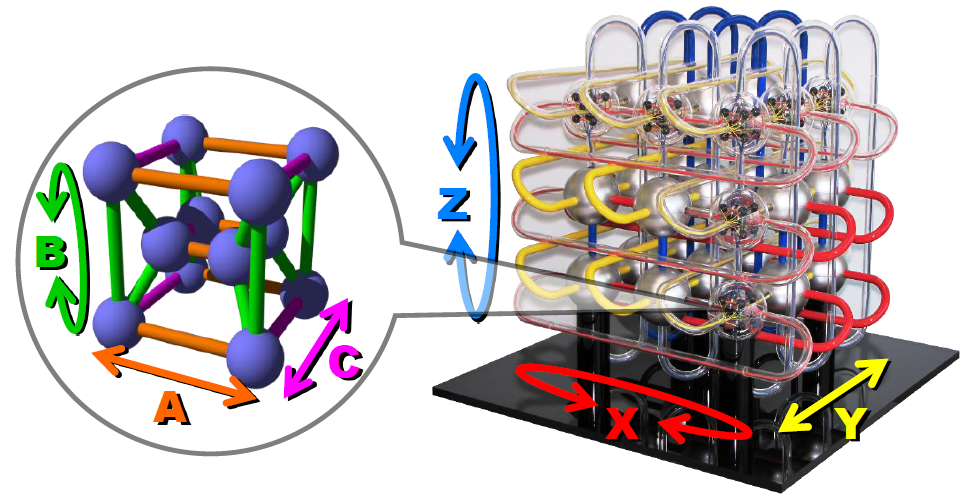
\includegraphics[width=.8\textwidth,height=.4\textwidth]{tofu.png}
\caption{Tofu模块和6D Mesh/Torus结构\upcite{tofu}}
\label{tofuto}
\end{figure}

\subsection{高性能互连网络}

E级高性能计算机系统的研制和应用面临巨大的挑战,
对高性能互连网络来说则面临更大的挑战。
高性能互连网络是高性能计算机系统的重要组成部分,
其主要功能是完成计算节点I/O 节点之间的通信。
随着处理器性能按照摩尔定律提升、
计算系统规模的按照指数级增长,
互连网络越来越成为影响系统性能的主要因素\upcite{johnkim}。
高性能互连网络主要由四个重要部分构成:
拓扑结构,路由算法,拥塞控制以及物理器件。
拓扑结构决定了报文在网络中最短跳步数、
节点间可用的总路径数和二分带宽,
路由算法则决定了报文在网络中的实际跳步数。
物理器件主要指通过拓扑结构相连并封装在机柜内的路由器和物理链路。
实际高性能互连网络通信则是依靠路由算法和拥塞控制机制保证。
除此之外,制约一个高性能互连网络的设计还有
很多因素\upcite{duato2002interconnection}。
主要因素介绍如下:

\textbf{网络性能}消息延迟和网络的吞吐率是网络性能的主要指标。
消息延迟是指消息在源节点开始发送的时间与目的节点接收消息的时间之差。
消息延迟直接影响处理器和存储的使用。
吞吐率则是在单位时间内,网络所能传输最大的信息量。
因为成本开销等原因,网络容量不是一个无底洞,
一旦饱和网络不会再传输新注入的消息,
这严重限制了系统的性能。
这两个指标跟网络拓扑结构的网络直径和链路容量紧密相关。

\textbf{灵活性和扩展性}一个灵活的网络,在扩大或者缩小规模的同时,
相应的带宽需求也按需求按比例增减,以保证性能不降低。
否则,带宽将成为系统瓶颈,降低系统效率。
同时,在物理器件约束下,网络仍然能够支持良好的扩展性,并保证网络性能。

\textbf{应用负载}网络可以根据应用负载的不同将网络中的节点或者链路划分成多个子网,
使得应用负载之间互相不影响性能。
同时,这也是出于安全因素的考虑。

\textbf{物理封装和器件约束}结合实际物理封装因素考虑
如何保持高性能互连网络拓扑本身的优良特性是设计高性能互连网络拓扑的重要问题。
物理封装有两个主要限制影响拓扑设计,一是缆线的长度和数量。
随着光纤技术的发展,机柜内部因为距离较短采用电信号传输,
机柜之间则采用光纤保证长距离的通信质量。
随着系统规模的增大,不仅缆线的数量增加使得物理封装难度增加,
由于机柜数的增加,缆线长度也因此增加而造成网络延迟增加,
如光纤传输延迟为每米5 纳秒。
第二个限制因素则是芯片的带宽和引脚数。
芯片的带宽和引脚数受限于芯片的面积,
在高阶路由器和光纤技术等器件发展不成熟时期,
互连网络受器件约束只能采用节点度数小,
网络直径大的结构,如经典的$k-ary$ $n-cube$结构。
随着工艺的进步,高阶路由器等器件的技术已成熟,
大规模低直径高性能互连网络成为高性能互连网络的主要结构。
除了此之外,简单性和可维护性都跟拓扑设计紧密相关的。
一个好的高性能互连网络拓扑结构一定是易构造,易维护的。

\textbf{可靠性} 为了保证网络性能,高性能互连网络是无损网络,
不支持丢包和重传。
因此,高性能互连网络的可靠性是保证网络传输的重要指标。
一旦发生有错误发生,网络中有多条可选路径保证传输不受影响。
而且,某条链路或者节点发生错误,网络的连通度不受影响等,
都是设计网络结构的时候需要考虑的场景。

\textbf{成本能耗开销} 随着系统规模的增加,
路由器个数和缆线数量的增加,都大大增加了成本和能耗的开销。
尤其,在能耗方面,若是随着规模的增加而线性增长,
将无法完成E 级高性能计算机系统的开发。
因此,在设计网络拓扑结构时,成本能耗开销起着决定性的作用。

\subsection{研究现状和不足}

本节主要回顾国际上在高性能互连网络设计方面的相关工作。
自高性能计算机系统发展以来,在HPCA、ISCA、 SC、 ICS等高性能领域顶级会议上,
高性能互连网络一直都是热点研究方向。
Intel、Cray、IBM、Bull、Mellanox等公司以及
许多研究小组都在关注和致力于研究高性能互连网络,
针对高性能互连网络的拓扑结构设计,路由算法及拥塞控制等方面进行研究。

随着对系统规模的需求增大,以及高阶路由器结构和光纤技术的发展,
大规模高性能互连网络采用低直径拓扑结构成为高性能互连网络的发展趋势。
在高性能计算机系统发展早期,
大部分高性能计算机系统的互连网络采用的要么是树形或者是
$k-ary$ $n-fly$蝶形等间接网络结构,
要么是$k-ary$ $n-cube$直接网络结构。
这些结构的特点都是使用端口数较小的交换机通过多级或者笛卡尔积的方式构建网络。
2007年,Kim等人在ISCA顶级会议上提出了使用高阶路由器搭建大规模
高性能互连网络低直径拓扑结构Flattened Butterfly\upcite{Flattenedbutterfly},
将高阶路由器替代传统的低阶路由器,从而减少路由器数量和降低网络直径。
之后,该组在2008年的ISCA会议上提出新型
高性能互连网络Dragonfly\upcite{dragonfly}结构和
2009年的超级计算机顶级会议SC上提出可灵活配置的HyperX结构\upcite{hyperx},
不仅充分利用高阶路由器的特点还将光纤运用在拓扑结构的不同层次。
至此,使用高阶路由器成为构建高性能互连网络新型拓扑结构的主要手段。
Cray、IBM等大公司也开始使用高阶路由器搭建高性能计算系统,
如Cray公司的Cascade系统\upcite{cascade}和IBM的PERCS系统。

在高性能互连网络拓扑结构方面,
Koibuchi所在的研究小组在2012年的ISCA会议上提出了
使用高阶路由器搭建随机拓扑\upcite{acaserandom},
其不仅网络直径低,平均最短路径小,还可以支持任意的网络规模。
但是,随机拓扑在物理布局中,面临缆线长短不一,连线复杂等不足,
2013年的HPCA会议上他们小组提出layout\-conscious的随机拓扑结构\upcite{fsorandom},
根据实际物理降低缆线的长度减少系统构建的开销。
2015年的HPCA 会议上,他们小组提出在机柜上摆放自由光设备,
根据不同应用的负载,在随机拓扑上添加自由光链路以满足不同的链路需求。
2014年的SC会议上瑞士联邦理工的Besta和Hoefler利用代数图论的方法
构造出近似最优的大规模低直径拓扑Slim Fly\upcite{slimfly}。
Slim Fly结构在不受路由器端口数限制的条件下,相比其他结构,
不仅端口利用率高,而且获得较优的网络性能。
2015年SC会议上Kathareios等人提出一个性价比更高,
直径为2的拓扑结构OFT\upcite{costeffective2}。
在同样的成本开销下,OFT结构相比Slim Fly结构,拥有更好的可扩展性。

高性能互连网络的路由算法是高性能互连网络的研究重点。
一个拓扑即使具备再好的优良特性,
如果没有合适的路由算法也不能展现出优良的网络特性。
路由算法决定了拓扑结构的实际网络性能。
随着系统规模的增加,大规模低直径互连网络成为高性能互连网络的首选。
同时,给设计合适的路由算法带来巨大挑战。
Jiang等人在2009年ISCA会议上对Dragonfly结构提出
间接自适应路由通过本地链路间接反馈来解决全局链路的拥塞\upcite{indirect}。
随后,Garc$\'{\i}$a等人分析出现有的自适应路由算法在解决
Dragonfly结构全局链路拥塞问题的同时引入了本地链路的拥塞,
因此,提出On\-the\-fly路由算法解决全局和本地链路拥塞\upcite{On-the-Fly}的问题。
On\-the\-fly路由算法由于是自适应绕路路由,
如果采用虚通道隔离的方式避免死锁,
路由芯片需要增加虚通道数目而增加缓存资源和控制单元。
不仅会增加了成本开销而且受芯片面积限制。
如果采用逃逸子网的方式避免死锁,
逃逸路径较长会严重影响网络性能。
因此,Garc$\'{\i}$a 等人提出了OFAR-CM\upcite{OFAR-CM}、
RLM\upcite{Rlmolm}和OLM\upcite{Rlmolm}解决On\-the\-fly路由算法的问题,
减少虚通道数量并保证网络性能。
Won等人在2015年HPCA会议上提出了避免
Dragonfly远端拥塞的路由算法\upcite{ofc},
通过添加历史窗口观察正在链路上传输的报文以判断应该走最短路径还是非最短路径。

拥塞控制机制对于高性能互连网络,重要性不低于路由算法。
Kim等人在\upcite{cbcm}中指出,路由算法是解决网络中链路拥塞,
拥塞控制机制则是解决终端拥塞。
路由算法和拥塞控制机制两者密切相关,
相互作用,相互影响,结果都是作用在网络性能上。
传统的Explicit Congestion Notification(ECN)
拥塞控制机制已经广泛使用在高性能互连网络,
如在InfiniBand Architecture\upcite{ecn1}\upcite{ecn2}\upcite{ecn3}。
但是,ECN机制对参数敏感,对拥塞情况反馈时间长,
不能准确及时的对拥塞采取措施。
尤其,高性能互连网络是一个无损网络,不允许网络中有丢包现象,
如果网络中发生拥塞,对网络性能影响巨大。
因此,Kim等人提出的CBCM 策略\upcite{cbcm}针对反馈时间长,
参数敏感等缺点做了有效的改进,
通过引入竞争度的概念,及时监测拥塞并作出反馈。
Jiang等人则提出了预约的方式主动避免终端拥塞\upcite{srp}\upcite{crp}\upcite{lhrp}。
除此之外,还有研究者把解决拥塞的关键放在降低Head-of-Line Blocking(HoLB)
出现概率,如FlexVC\upcite{flexvc}以及Y$\'{e}$benes等人的
相关研究 \upcite{Y2017Providing}\upcite{Y2017An}\upcite{Y2018Head},
有效的利用虚拟通道减少HoLB的发生。

E级计算时代即将到来标志着高性能互连网络也将要进入一个新时代,
但是,这同时也给高性能互连网络现有技术带来了巨大挑战。
目前的高性能互连网络新型拓扑结构无法同时满足E级计算规模、
灵活性、器件约束、物理封装、网络性能、应用负载等需求,
已有的路由算法和拥塞控制机制也随着拓扑规模、
网络直径、 应用负载等变化面临新的挑战。

\section{论文的主要工作}
本文面向高性能互连网络,
针对当前新型高性能互连网络在物理器件约束下如何满足E级计算系统网络规模、
灵活性以及应用负载的需求,路由算法如何解决缓存资源利用率低等问题,
分别对灵活的、满足应用负载的新型高性能互连网络以及
高效利用缓存资源的路由算法等具有挑战性的问题进行深入的研究,
论文的主要工作总结如下:

(1)针对在E级计算的挑战下,
因路由器端口数约束使当前高性能互连网络的灵活性及网络性能方面的不足,
提出一种灵活端口数的高性能互连网络新型拓扑结构Galaxyfly。
Galaxyfly利用代数图论有限域的方法构造而成。
在保持低直径的情况下,Galaxyfly可以达到网络规模和二分带宽的灵活权衡。
其降低了对高阶路由器端口数的要求,
可以使用较少的端口数去构建E级计算系统的网络规模。
针对Galaxyfly结构,不仅分析了可构造的配置并且评估了最短路径数量。
利用其代数图论的性质,设计了拥塞敏感的路由算法。
与其他新型高性能互连网络拓扑结构分别从性能、
成本和能耗三方面进行了实际物理布局的模拟和分析比较。
结果表明Galaxyfly相比其他结构,在不同的路由算法以及典型的通信模式下,
能够展现更优的性能,是一个适合构建E级计算系统的新型高性能互连网络拓扑结构。

(2)针对在E级计算的挑战下,
目前高性能互连网络的网络性能、可维护性以及物理封装方面的不足,
提出一种适合使用多芯光纤的高性能互连网络新型拓扑结构Bundlefly。
Bundlefly是一个低直径、可灵活扩展并且适合采用多芯光纤连接机柜之间的拓扑结构。
随着集成光模块板的发展,一根多芯光纤可以替代一捆传统的单芯光纤,
不仅可以降低光纤的使用成本还可以提高光纤的可维护性。
虽然Bundlefly的网络直径只有3,
但是其不仅能够充分利用多芯光纤来提高机柜间的通信带宽
还能降低高阶路由器的端口数的要求来支持E级系统的可扩展性。
通过分析和模拟,比较了Bundlefly和其他新型高性能互连网络拓扑结构,
Bundlefly能够完成更好的性能。

(3)针对目前高性能互连网络自适应路由算法对虚拟通道数量要求高以及
缓存资源利用均衡的不足,提出了一种标签路由算法Label-based Routing(LBR)。
LBR通过协同设计路由器微体系结构里的输入缓冲区模块和路由计算模块,
将路由计算引入缓冲区模块,
根据网络状态对路由报文做标记。
LBR不仅降低了死锁避免政策对虚拟通道的需求,
还均衡使用缓存资源并有效实现完全自适应路由。
通过模拟在Dragonfly结构上评估了LBR的性能并与其他拓扑结构进行了对比。
实验表明,在大部分通信模式下,LBR优于别的路由算法近10\%-35\%。

\section{论文的组织结构}

本文紧紧围绕高性能互连网络新型拓扑结构和路由算法进行优化设计,
本文共分为六章。
论文组织框图如图\ref{orgth}及各章节主要内容介绍如下:


\begin{figure}[htp]
\centering
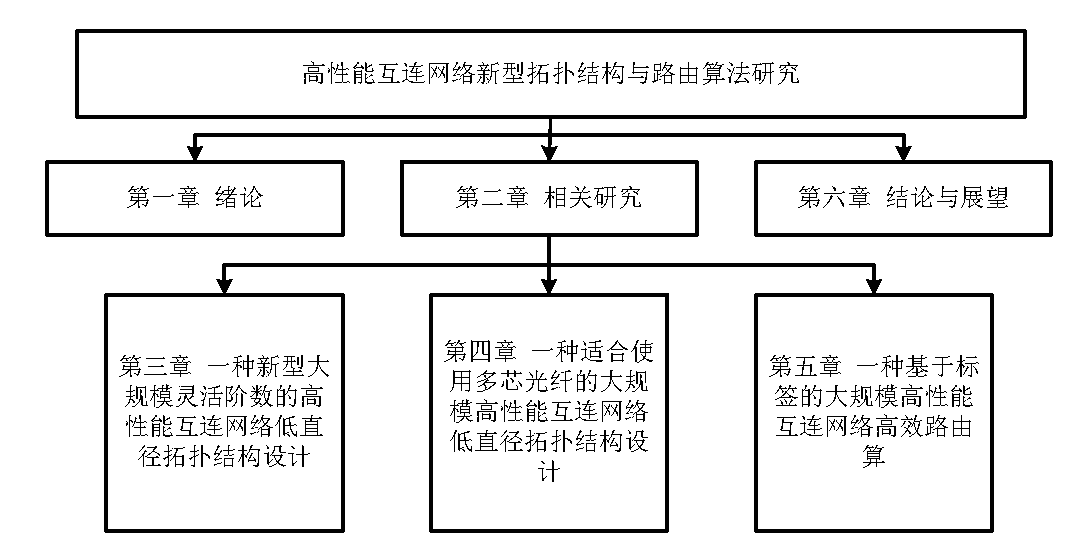
\includegraphics[width=.88\textwidth,height=.45\textwidth]{Visio-org_th.eps}
\caption{论文组织框图}
\label{orgth}
\end{figure}

第一章绪论,首先对高性能计算以及高性能计算机进行介绍,
并论述了高性能互连网络的研究意义以及高性能互连网络设计需要考虑的因素,
然后对高性能互连网络的研究现状以及不足进行分析,
最后简述了本文的主要研究内容和组织结构。

第二章介绍了本文的研究技术背景,包括物理器件对高性能互连网络设计的影响,
高性能互连网络新型拓扑结构,
高性能互连网络路由算法及高性能互连网络拥塞控制机制。

第三章提出了一种灵活端口数的高性能互连网络新型拓扑结构Galaxyfly。
首先详细介绍了Galaxyfly拓扑结构的构造方法,
然后对Galaxyfly结构的灵活性、可构造配置、
最短路径数以及容错性进行了详细的理论分析,
之后描述了Galaxyfly结构的路由算法。
最后通过模拟仿真对Galaxyfly的网络性能进行验证。

第四章提出了一种适合多芯光纤的高性能互连网络新型拓扑结构Bundlefly。
首先详细介绍了Bundlefly拓扑结构的构造方法,
然后对Bundlefly结构的网络直径、可扩展性、二分带宽、最短路径数、平均最短路径
以及容错性进行了详细的理论分析,
之后描述了Bundlefly结构的路由算法。
最后通过模拟仿真对Bundlefly的网络性能进行验证。

第五章提出了一种基于标签的高性能互连网络路由算法Label-based Routing。
首先详细介绍了Label-based Routing算法的整体架构,
然后论述Label-based Routing算法的缓冲区、
路由算法以及虚拟通道分配机制,
最后通过模拟仿真对Label-based Routing的性能进行验证。

第六章结论与展望,对全文的研究内容和主要工作进行总结,并对后续的工作进行展望。

\chapter{相关研究工作}
本章介绍高性能互连网络设计的相关背景知识。
首先介绍了物理器件对新型高性能互连网络的影响,
之后介绍了典型的高性能互连网络拓扑结构和路由算法。

\section{物理器件对高性能互连网络的影响}
传统的高性能互连网络拓扑大致分为两类
,一类是以$k\textrm{-}ary$ $n\textrm{-}fly$蝶形网络为代表的间接网络,
如图\ref{butterfly}所示。
$k\textrm{-}ary$ $n\textrm{-}fly$结构中,节点度数为$2k$,采用单向链路,
网络直径为$n-1$,网络规模为$k^n$。
一类是以$k\textrm{-}ary$ $n\textrm{-}cube$网络为代表的直接网络,
如图\ref{torus} 所示。
$k\textrm{-}ary$ $n\textrm{-}cube$结构中,节点度数为$2n$,采用双向链路,
网络直径为$n \lfloor k/2 \rfloor$,网络规模为$k^n$。
%% FIXME $n(\lfloor\frac{k}{2}\rfloor)$
当$k=2$时,$k\textrm{-}ary$ $n\textrm{-}cube$结构就是经典的超立方体(Hypercube)结构,
是第一代高性能计算机的主要拓扑结构。
如Intel iPSC/2\upcite{ipsc2}、 NCUBE/10\upcite{ncube}、
SGI Origin 2000\upcite{sgi2000} 等系统均采用了Hypercube结构,
因为其具有正则性、对称性、强容错性以及可嵌入性等特点。
当$k=n$时,$k\textrm{-}ary$ $n\textrm{-}fly$结构和$k\textrm{-}ary$ $n\textrm{-}cube$结构规模一样,
节点度数一样,但是$k\textrm{-}ary$ $n\textrm{-}cube$结构的网络直径大约是
$k\textrm{-}ary$ $n\textrm{-}fly$结构的$k/2$倍。
$k\textrm{-}ary$ $n\textrm{-}fly$ 结构拥有更小的网络直径,
但是,路径唯一性及负载不均衡是限制其扩展的主要原因。

%% FIXME annotate these two figures with concreate n/k values?
%% FIXME also more explanation needed in the text?
\begin{figure}[htp]
  \centering
   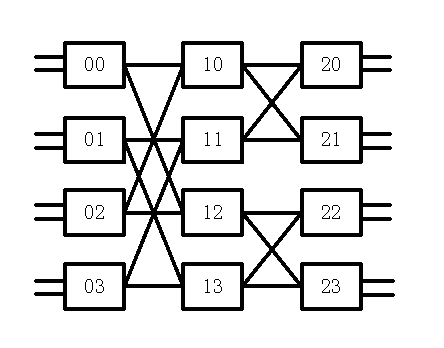
\includegraphics[width=.48\textwidth,height=.38\textwidth]{Visio-butterfly.eps}
    \caption{$k\textrm{-}ary$ $n\textrm{-}fly$结构}
    \label{butterfly}
\end{figure}

\begin{figure}[htp]
  \centering
   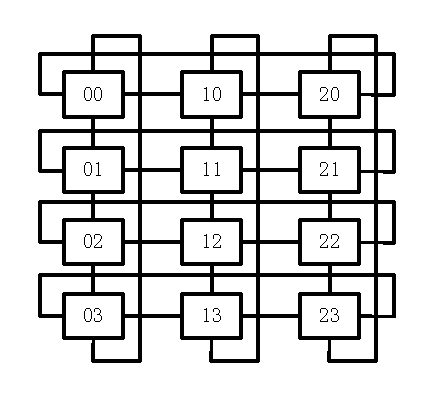
\includegraphics[width=.44\textwidth,height=.38\textwidth]{Visio-torus.eps}
      \caption{$k\textrm{-}ary$ $n\textrm{-}cube$结构}
      \label{torus}
\end{figure}

%% FIXME 10Gb/s or 10GB/s
上世纪90年代,路由芯片引脚带宽上限约为10Gb/s,
%% FIXME 端口数受限是因为引脚带宽低?
路由芯片也因此端口数受限制。
传统的高性能互连网络只能采用低节点度的拓扑结构。
随着半导体和集成电路的发展,路由芯片的引脚带宽增加,芯片端口数也随之增加。
如Cray公司推出的端口数为64的YARC路由芯片
\upcite{yarc}\upcite{blackwindow}、2010年HOTI
会议上提出的48端口Gemini芯片\upcite{cascade}、
2015年HOTI会议上提出48端口的Intel Omni-Path芯片\upcite{omni}以及
Mellanox 公司最新推出的Quantum 200G HDR InfiniBand Switch\upcite{quantum}。
相比拥有较少宽带宽端口的路由芯片,
采用拥有更多窄带宽端口的路由芯片搭建高性能互连网络可以降低网络的延迟和成本开销。
根据Kim的推导,低负载下报文的网络延迟为$T=T_h+T_s=Ht_r+L/b$,
其中$H$是报文的跳步数,$t_r$是每一跳经过路由器的延迟,$L$是报文的长度,
$b$则是链路的带宽。
在规模为$N$的网络中,若使用端口数为$k$的路由芯片($k$个输入通道加$k$个输出通道),
其跳步数最少为$2log_kN$。
若芯片的总带宽为$B$,则$b=B/2k$。
那么网络延迟为$T=2t_rlog_kN+2kL/B$,对$k$求导,
当$dT/dk=0$时可得到网络延迟$T$取最小值时端口数$k$满足$klog^2k=Bt_rlogN/L$。
随着网络规模$N$增加,路由芯片的最佳端口数$k$也随之增加。
%% 不要一句话不停重复地说……
%% 因此,基于高阶路由器设计的高性能互连网络成为高性能互连网络设计的主流趋势。
随着路由器端口数的增加,基于高阶路由器的网络拓扑结构相继被提出,
如Flattened Butterlfy \upcite{Flattenedbutterfly}、Dragonfly \upcite{dragonfly}、
HyperX \upcite{hyperx}等。
相比传统的高性能互连网络拓扑结构,
基于高阶路由器设计的网络拓扑结构不仅可以在降低网络直径的前提下支持更大的网络规模,
还可以减少路由器的数量。
Kim曾预测,未来几年内将会出现数百个端口的路由芯片,
2010年单芯片的总带宽会突破20Tb/s\upcite{yarc}\upcite{blackwindow}。
但是,实际上目前最新的商用芯片总带宽只能达到16Tbps\upcite{quantum}。
总体上,虽然路由芯片取得了长足的发展,
但采用目前的高性能互连网络仍远不足以构建E级计算系统,
如何利用当前商用高阶路由芯片搭建E级计算系统已经成为高性能互连网络研究的关键问题。

光纤技术的发展使得高性能互连网络在实际部署中引入光缆代替部分电缆。
大规模低直径的新型高性能互连网络相比传统的高性能互连网络,
拥有更多的全局链路以降低网络直径。
对全局链路采用光纤部署,不仅在性能上有优势,而且在能耗上独立于榄线的物理长度。
研究表明,10米以内的链路,采用光纤的成本相比电缆的成本要高,
而10米以上的链路,
则采用电缆的成本要比光纤的高\upcite{dragonfly}。
因此,为了降低系统成本,
Dragonfly结构在保证网络直径低的前提下,
每个超级节点只引出一条全局链路连接相邻超级节点\upcite{dragonfly}。
但是,E级计算系统的应用负载复杂多样,
除了对网络结构的局部性有要求外,全局通信将更加频繁,
若只保证超级节点间
只有一条全局链路已不能满足应用负载的需求。
从边缘可插拔光纤收发器到主板集成光模块的转变\upcite{BOA},
多芯光纤(Multicore Fiber)\upcite{MCF}的出现
给高性能互连网络设计带来了新的契机,
这给提升实际部署中机柜间通信带宽提供了更多空间。
多芯光纤,如图\ref{mcf}所示,实际上就是一条光缆里有多个纤芯的光缆,
可以通过分线器分成多个单芯光纤。
一条多芯光纤相比同等纤芯数的一捆单芯光纤,
不仅成本上更加经济,而且维护上更加容易。
因此,如何在高性能互连网络中更好地利用多芯光纤,
有效提升全局通信带宽并保证可扩展性,提高可维护性是构建
E级计算系统的关键问题。

\begin{figure}[htp]
  \centering
    
\includegraphics[width=.48\textwidth,height=.38\textwidth]{Visio-SCF.eps}
    \caption{单芯光纤}
    \label{scf}
\end{figure}

\begin{figure}[htp]
  \centering
    
\includegraphics[width=.48\textwidth,height=.38\textwidth]{Visio-MCF.eps}
      \caption{多芯光纤}
       \label{mcf}
\end{figure}

\section{高性能互连网络拓扑结构}

\subsection{Fat tree}
Fat tree\upcite{fattree}是最早的大规模低直径高性能互连网络拓扑结构。
国防科技大学自主研制的天河一号和天河二号高性能计算机均采用Fat tree结构。
Fat tree是一个灵活性和扩展性都较优的拓扑结构,
最大的特点在于随着网络规模的增加,二分带宽也随之等规模增加。
其可以看成是两个$k\textrm{-}ary$ $n\textrm{-}fly$结构合并而成,
如图\ref{fattree}所示由两个图\ref{butterfly}合并而成,采用双向链路。
%% FIXME use concreate n/k
两个蝶形结构分别起到负载均衡和控制输入输出的作用,
因此,Fat tree继承了蝶形结构网络直径低的优点,
并且可以有效避免蝶形网络路径唯一和负载不均衡等缺点。
Fat tree的节点度数为$2k$,网络直径为$2(n-1)$,
网络规模$2k^n$,且需要$(2n-1)k^{n-1}$个路由器。
%% FIXME 如何用n/k定义胖树?
\begin{figure}[htp]
  \centering
    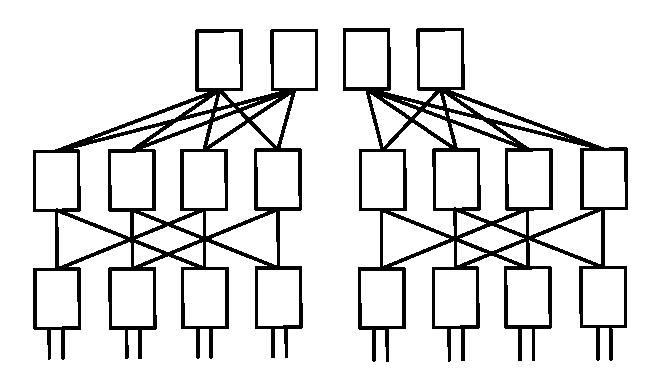
\includegraphics[width=.48\textwidth,height=.38\textwidth]{Visio-fattree.eps}
    \caption{Fat tree结构}
     \label{fattree}
\end{figure}

\subsection{Flattened Butterlfy}

Flattened Butterfly\upcite{Flattenedbutterfly}是2007年Kim等人
在ISCA会议上提出的一个性价比较高的高阶互连网络。
Flattened Butterfly结构充分利用高阶路由器提供的丰富链路特性,
使得$k\textrm{-}ary$ $n\textrm{-}cube$结构中每一维上的路由节点都是全互连,
其节点度为$(n+1)(k-1)+1$,网络直径为$n$,网络规模为$k^{n+1}$。
%% FIXME 如何用n/k定义FB
Flattened Butterfly利用高阶路由器,
不仅有效解决了$k\textrm{-}ary$ $n\textrm{-}cube$结构网络直径长的问题
而且通过合并$k\textrm{-}ary$ $n\textrm{-}fly$结构中的路由器,有效降低了路由器的数量。
如图\ref{flattenedbutterfly}所示,图左是$k\textrm{-}ary$ $n\textrm{-}fly$结构,
图右是合并了蝶形网络中每一层的路由器的Flattened Butterfly。
与Fat tree相比,当搭建同样规模和同样直径的网络时,
Flattened Butterfly可以节省近一半的链路。

\begin{figure}[htp]
  \centering
    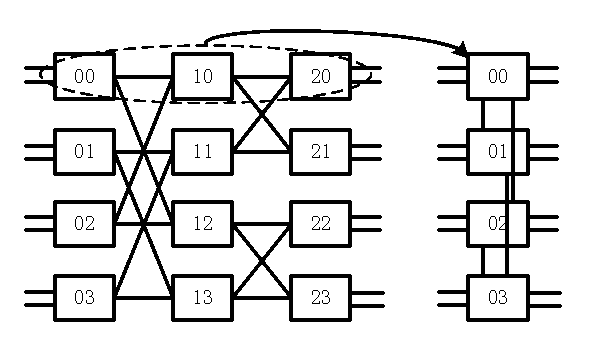
\includegraphics[width=.56\textwidth,height=.35\textwidth]{Visio-flattenedbutterfly.eps}
    \caption{Flattened Butterfly结构}
    \label{flattenedbutterfly}
\end{figure}

2009年SC会议上提出的HyperX\upcite{hyperx}
结构实际上是基于Flattened Butterfly结构的扩展结构,
是一个可以灵活配置的高阶互连网络。
HyperX同样是一个$k\textrm{-}ary$ $n\textrm{-}cube$结构,
但是每一维上的$k$值可以取不同值,
而且每个路由节点所连接的终端数以及每一维上的链路带宽都可以随意配比。
在网络规模、性能需求和能耗成本开销上,
这类可灵活配置的拓扑结构都更适合实际系统的需求。
Hypercube和Flattened Butterfly都是HyperX的特例。

%% FIXME 可能是因为第一章就没有把k-ary n-cube和k-ary n-fly 解释清楚,
%% 后面的拓扑结构感觉都没那么容易理解,以外行的眼光。

\subsection{Dragonfly}

Dragonfly\upcite{dragonfly}结构是一个有标志意义的高阶互连网络,
也是大规模低直经高性能互连网络的典型代表。
相比低阶互连网络,高阶互连网络拥有更多的全局链路,使用更多的长缆线。
为了解决高阶互连网络长缆线成本开销的问题,Dragonfly利用层次化的结构有效
减少了全局链路的数量并同时支持较大的网络规模和较低的网络直径。

Dragonfly具体构造是将$a$个高阶路由器通过全互连的方式相连成虚拟的更高阶超级节点,
每个路由节点引出$a-1$条本地链路连接同一个超级节点内的其他路由节点,
如图\ref{dragonfly}中虚线框所示。每个路由器引出$h$条全局链路
链接其他超级节点内的路由节点。
在全局网络中,虚拟的更高阶超级节点两两之间至少有一条链路相连,
如图\ref{dragonfly}中虚线框之间的连线所示。
通过在不同层次的网络中采用全互连结构,Dragonfly的网络直径只有3。
相比同样规模和同样节点度数的Flattened Butterfly结构,
Dragonfly结构可以节省近一半的全局链路。

\begin{figure}[htp]
  \centering
    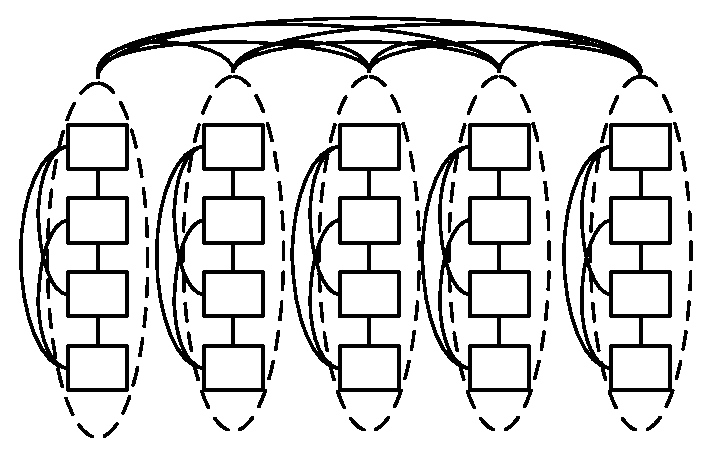
\includegraphics[width=.56\textwidth,height=.35\textwidth]{Visio-dragonfly.eps}
    \caption{Dragonfly结构}
       \label{dragonfly}
\end{figure}

在2017年HiPINEB会议上提出的Dragonfly+\upcite{Dragonfly+}
拓扑结构是在Dragonfly结构的基础上进行扩展优化,
使用直径为2的树形结构替代Dragonfly结构超级节点内的全互连网络,
同时保持网络直径为3,
Dragonfly+使用图\ref{dragonfly+}所示的结构替代图\ref{dragonfly}中的超级节点。
使用相同端口数的路由芯片搭建网络,
Dragonfly+结构可以支持的最大网络规模接近Dragonfly结构的4倍。

\begin{figure}[htp]
  \centering
    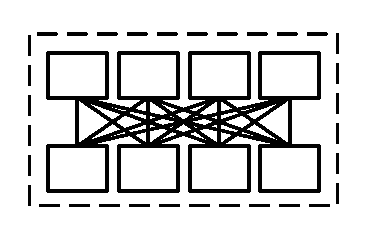
\includegraphics[width=.48\textwidth]{Visio-dragonfly+.eps}
    \caption{Dragonfly+结构中超级节点模块}
    \label{dragonfly+}
\end{figure}

\subsection{Slim Fly}
Slim Fly\upcite{slimfly}是一个近似最优的高性能互连网络拓扑结构。
Slimf Fly的设计目标是,在直径为2的前提下,
使用尽可能少的路由器端口数构造更大规模的拓扑结构。
Slim Fly结构是继Dragonfly结构之后又一个标志性拓扑结构,
其利用代数图论的构造方法,
满足了低直径大规模的要求,
而且在二分带宽和成本能耗以及容错性上都展现了较优的性能。

Slim Fly采用了代数图论里的MMS图\upcite{MMS}。
其构造取决于一个基本参数$q$,$q$是一个素数的幂,可以表示为
$q=4w+\delta$,其中$\delta \in \{-1,0,1\}$。
Slim Fly图是一个高对称性的结构,由两个子图构成,
%% FIXME 每个子图多少子组,每个子组多少节点,用符号表示。
%% 检查以下我理解的对不对,每个子组是不是q个路由节点?
每个子图内包括$q$个子组,每个子组包含$q$个路由节点。
在Slim Fly中,每个路由器引出$q-\delta$条链路连接同一个子组内的其他路由节点,
$q$条链路分别连接另一个子图中$q$个子组的路由节点。
如图\ref{slimflyone}所示,
Slim Fly中的每个路由节点用一个三元组$(a,x,y)$标识,
其中$a\in \{0,1\}$标识子图的编号,
$x,y\in\mathds{F}_q$分别标识在所在子图中子组的编号和
所在子组中路由节点的编号。

令集合$X$和$X'$表示有限域$\mathds{F}_q$的两个生成集\upcite{MMS}\upcite{GRMMS},
他们可以通过有限域$\mathds{F}_q$的生成元$\xi$
通过式\ref{equ:generator-sets0}和\ref{equ:generator-sets1}构造。
那么Slim Fly结构中的链路构造方式如下:
\begin{itemize}
\item 当且仅当$y-y' \in X$,路由节点$(0,x,y)$与路由节点$(0,x,y')$相连。
\item 当且仅当$y-y' \in X'$,路由节点$(1,x,y)$与路由节点$(1,x,y')$相连。
\item 当且仅当$y=x'x+y'$,路由节点$(0,x,y)$与$(1,x',y')$相连。
\end{itemize}

\begin{figure}
  \centering
    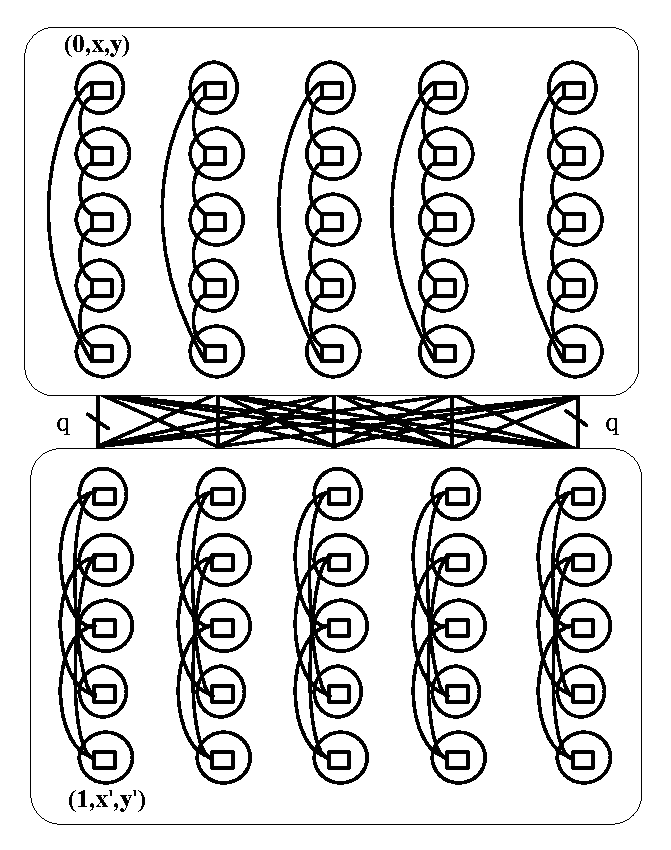
\includegraphics[width=.6\textwidth]{Visio-Slimfly_between.eps}
    \caption{Slim Fly结构}
    \label{slimflyone}
\end{figure}

\begin{equation}\label{equ:generator-sets0}
  X=
  \begin{cases}
    \{1,\xi^2,\ldots,\xi^{q-3}\}& q=4 \ell+1 \\
    \{1,\xi^2,\xi^4,\ldots, \xi^{2\ell-2},\xi^{2\ell-1},\xi^{2\ell+1},\ldots, \xi^{4\ell-3}\} & q=4 \ell-1 \\
    \{1,\xi^2,\ldots,\xi^{4l-2}\} & q=4 \ell
  \end{cases}
\end{equation}
\begin{equation}\label{equ:generator-sets1}
  X'=
  \begin{cases}
    \{\xi,\xi^3,\ldots,\xi^{q-2}\} & q=4 \ell+1 \\
    \{\xi,\xi^3,\xi^5,\ldots,\xi^{2\ell-1}, \xi^{2\ell},\ldots,\xi^{4\ell-4},\xi^{4\ell-2}\}\ \ \ \  & q=4 \ell-1 \\
    \{\xi,\xi^3,\ldots,\xi^{4l-1}\} & q=4 \ell
  \end{cases}
\end{equation}

%% FIXME 上面没说SF的全局网络是什么
在实际物理部署中,Slim Fly可以部署成全局网络是一个全互连网络。
分别位于相邻子图的两个子组封装成一个机柜,
那么任意两个机柜之间都有$2q$条链路,
%% FIXME 这句话在图中也体现不出来
如图\ref{slimfly}所示。

\begin{figure}[htp]
  \centering
    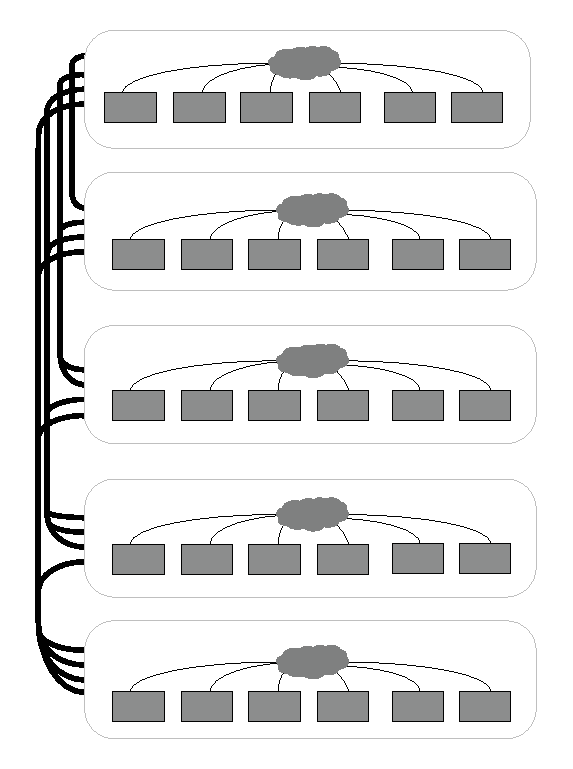
\includegraphics[width=.3\textwidth,height=.5\textwidth]{Visio-Slimfly.eps}
    \caption{Slim Fly结构的全局网络}
    \label{slimfly}
\end{figure}

在2015的SC会议上,两种网络直径为2的间接拓扑结构
OFT(two-level Orthogonal Fat-Trees)和MLFM(Multi-Layer Full-Mesh)
被提出\upcite{costeffective2},
分别如图\ref{oft}和\ref{mlmf} 所示。
在相同条件下,OFT相比Slim Fly和MLMF可以构造近似2倍规模的网络,
MLMF的可扩展性跟Slim Fly一样。
这三种拓扑结构的相同点就是平均每个终端都是消耗3个路由器端口和2条链路。
%% FIXME 这段话仅仅说OFT在规模上更好,但MLFM等于啥都没说。
%% 况且,OFT规模比SF大,那缺点呢?不都是tradeoff么。
%% 再况且,只说如图所是,还应该加一点对图的解释。

\begin{figure}[htp]
  \centering
    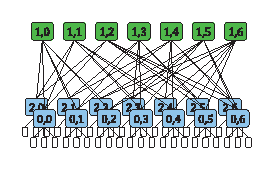
\includegraphics[width=.6\textwidth]{oft.eps}
    \caption{OFT结构\upcite{costeffective2}}
    \label{oft}
\end{figure}

\begin{figure}[htp]
  \centering
    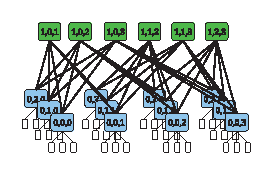
\includegraphics[width=.6\textwidth]{mlmf.eps}
    \caption{MLMF结构\upcite{costeffective2}}
    \label{mlmf}
\end{figure}

\subsection{随机拓扑}

除了前面介绍的规则拓扑外,
随机拓扑也是高性能互连网络新型拓扑结构的一个重要类型。
最早是在数据中心网络中提出使用小世界网络\upcite{smallworld}构造系统。
通过在规则拓扑结构上添加随机链路构造出具有小世界网络特性的随机网络,
图\ref{sw2d}展示了一种在2D Torus结构上添加随机链路构小世界网络形成的拓扑结构。
在约束节点度情况下,具有小世界网络特性的网络
不仅可以拥有较短的网络直径,而且具备较高带宽和较短平均最短路径。
Singla等人提出将Jellyfish\upcite{Jellyfish}
运用在top-of-rack(ToR)交换机之间。
Jellyfish是一个绑定节点度的随机图拓扑结构,
不仅可以支持任意规模,而且相比同样配置的Fat tree,
可以支持更多的节点并提供至少一样的带宽。
Valadarsky等人指出当前最新的拓扑结构,如Slim Fly和Jellyfish,
都是expander图\upcite{xpander}。
但是,在性能上这些拓扑结构还不能达到近似最优,并在它们扩展上和部署上都存在困难。
因此,他们提出Xpander结构\upcite{xpander},不仅提供近似最优的性能,
而且切实提高了部署可行性。
Xpander是一个灵活扩展的拓扑结构,
每个节点表示一个ToR交换机,每个节点有$d$个端口连接其他ToR交换机,
扩展则以包含$d+1$个节点的全互连图为单位进行。
通常情况下,Xpander结构都是通过翻倍的方式扩展,
但是Xpander也支持线性扩展来满足任意规模。
图\ref{xpander}给出了$d=2$的Xpander结构,
即,每个节点有2个端口连接其他节点,
以3个节点的全互连图为单位扩展成节点为6的Xpander结构。
%% FIXME 从这个图上看不出是怎么扩展的,也看不出d表示什么

\begin{figure}[htp]
\centering
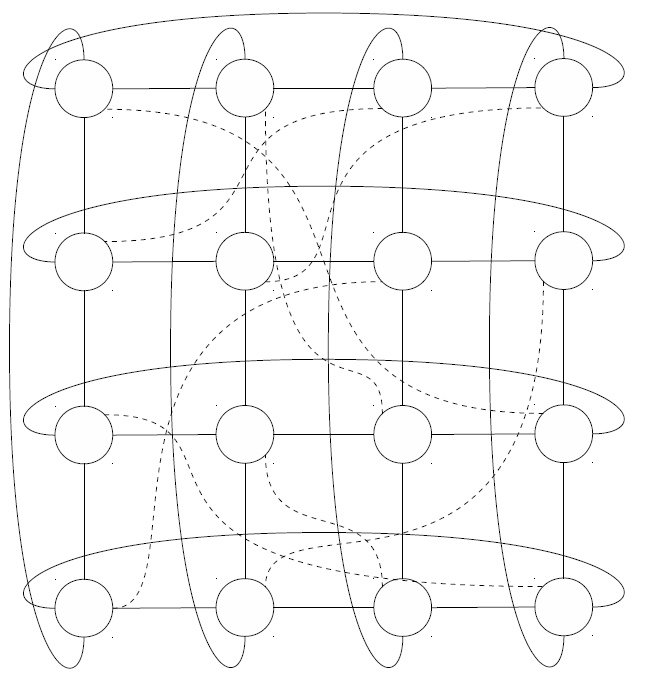
\includegraphics[width=.5\textwidth]{sw2d.png}
\caption{小世界网络\upcite{smallworld}}
\label{sw2d}
\end{figure}
%% FIXME 这个图的线太细了

\begin{figure}[htp]
\centering
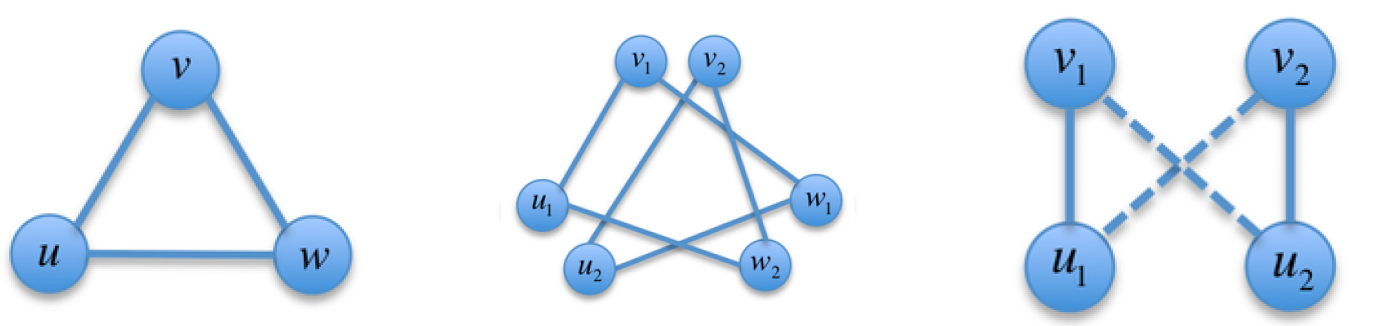
\includegraphics[width=.8\textwidth]{xpander.png}
\caption{Xpander结构\upcite{xpander}}
\label{xpander}
\end{figure}

Koibuchi等人\upcite{acaserandom}首先提出在高性能互连网络中采用随机拓扑结构
以满足系统延迟低、灵活扩展等需求。
具体构造方式类似于小世界网络,在圆环拓扑结构上添加随机链路,
可以支持任意规模的网络。
在2013年的HPCA会议上,
Koibuchi等人在之前提出的随机拓扑上进行了优化\upcite{layoutrandom},
加入了物理布局的考虑,限制了缆线的长度。
之后在2015年的IPDPS会议上他们研究组提出Skywalk拓扑结构\upcite{skywalk},
其进一步约束随机链路在实际物理布局的三维结构中的连接方式
来降低链路延迟对网络延迟的影响。
在2015年的HPCA会议上,
他们研究组提出在机柜间利用基于自由空间光(FSO)的随机链路来
降低网络延迟并优化任务分配\upcite{fsorandom}。
如图\ref{fso}所示,通过在机柜上部署FSO设备,
以便根据任务负载添加FSO通信链路以优化性能。

虽然随机拓扑可以提供较短的网络直径和平均最短路径,
并可以灵活支持任意规模,
但是,路由算法是限制随机拓扑应用于实际系统部署的主要原因之一。
由于随机拓扑结构只能通过路由表的方式进行路由,
随着网络规模的增长,路由表规模呈指数级增长,这是在实践中难以接受的。

\begin{figure}[htp]
\centering
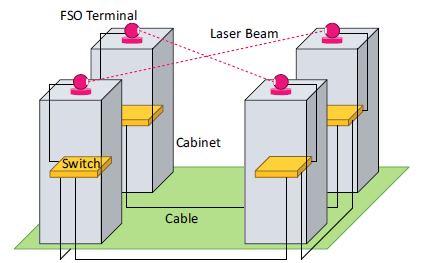
\includegraphics[width=.7\textwidth]{fso.png}
\caption{添加FSO链路的高性能互连网络\upcite{fsorandom}}
\label{fso}
\end{figure}

\section{高性能互连网络路由算法}

拓扑结构和路由算法是紧密相关的,路由算法决定了拓扑结构的实际网络性能。
路由算法除了决定报文在拓扑结构的路径也同时影响网络
在实际通信下的拥塞情况以及网络的死锁避免策略。
虽然在高性能互连网络中,新型拓扑的连接方式多种多样,
但是,相同点都是网络规模大且直径低。
这个相同点造成了新型拓扑结构只有少量的冗余最短路径且部分关键链路使用频率高。
如Slim Fly\upcite{slimfly}结构中只有
极少量的节点对之间的最短路径多于一条,
Dragonfly\upcite{dragonfly}结构中超级节点之间的链路负载很中,容易造成网络的拥塞。
在实际通信中,为了满足不同的应用负载,
使用自适应路由算法是提升网络性能、解决网络中链路拥塞的主要方法之一。
然而,在新型拓扑结构中只能使用非最短路径代替最短路径,
这不仅给自适应路由算法的性能造成影响,
同时也给死锁避免策略带来成本开销和工艺设计等挑战。

Dragonfly结构是高性能互连网络的新型拓扑结构典型代表之一,
学术界针对其结构特点提出了很多路由算法。

最短路径路由(MIN)是Dragonfly结构上最简单和最基本的路由算法\upcite{dragonfly}。
使用最短路径路由最多只需3跳就能将报文从源路由节点传送到目的路由节点,
即:源路由节点所在的超级节点内的本地链路、
源超级节点和目的超级节点的全局链路和目的超级节点的本地链路。
因为Dragonfly的结构特点,本地链路和全局链路的VC可以复用,
因此MIN算法至少需要两条VC来避免死锁。

非最短路径路由又称Valiant路由算法(VAL)\upcite{dragonfly},
是针对高负载流量提出的路由算法。
报文先选择一个中介节点作为第一个目的路由节点,
当通过MIN从源路由节点到达中介节点后再通过MIN 从中介节点到达目的路由节点。
这样做的好处是,缓解高负载流量对全局链路的过度请求。
具体在实施时Valiant路由算法可划分为两种,
一种(VAL)是以中介节点所在的超级节点为第一目的地,
只要报文到达中介节点所在的超级节点就将目的地换成真正的目的路由节点。
第二种(VAL$_n$\upcite{overcomefarend})则是按前面介绍的以中介节点为第一目的地。
第一种VAL最长需要经过5跳到达终点,途
经3条本地链路和2条全局链路。
VAL$_n$则最长需要经过6跳到达终点,途经3条本地链路和3条全局链路。
两种算法都至少需要3条VC来避免死锁。

在均衡随机通信模式下,VAL相比MIN,不仅跳步数翻倍,
吞吐率也会相应减半。而在密集高负载的最差通信模式下,
MIN则会造成全局链路的严重堵塞。
根据网络状态选择走VAL机制或是MIN机制是均衡全局自适应路由算法
(UGAL)的主要机制\upcite{dragonfly}。
网络状态则由路由端口缓冲区队列长度和报文的跳步数共同决定。
由于UGAL最长跳步数由VAL机制决定,
因此,UGAL同VAL一样至少需要3条VC来避免死锁。

上述四种Dragonfly结构路由算法存在一个共同的问题,那就是不能及时感知并反馈全局链路的拥塞状况。
因此,有研究提出间接自适应路由算法\upcite{indirect}来迅速对全局链路的拥塞作出反馈。
图\ref{dragonflyir}展示了四种不同的间接自适应路由算法。
第一种间接自适应路由算法CRT (Credit Round Trip),
通过感知本地链路的信用反馈延迟来判断全局链路拥塞情况使得UGAL算法及时对拥塞做出
反馈,如路由器R0通过本地链路给路由器R1发送报文再通过全局链路给路由器R2发送报文,
路由器R1给路由器R0的信用反馈需等到路由器R2的信用反馈返回到R1才能发送。
CRT通过背压的方式获得全局链路的拥塞信号,
但是可能会造成本地链路拥塞。
第二种间接自适应路由算法PAR(Progressive Adaptive Routing),
如图\ref{dragonflyir}所示,在源超级节点根据当前
拥塞情况作出路由决策,选择MIN或者VAL。
这种方法在发现全局链路拥塞时不会将拥塞情况反馈给源路由器。
该算法会多走一跳本地链路,在使用VC隔离的方法来避免死锁时,需要多一条VC。
PAR可以扩展到在经过的每一个超级节点内部都根据当前网络状态选择MIN或者VAL。
第三种间接路由算法PB(Piggyback),
如图\ref{dragonflyir}所示,
通过给相邻节点广播全局链路的拥塞状态作出路由选择。
具体实现则需要在每个报文上都增加一个记录链路状态的向量位。
每个路由器都需要维护同一个超级节点内全局链路的状态信息。
该算法缺点是路由器需要维护全局链路拥塞信息的更新。
第四种间接路由算法RES(Reservation),
如图\ref{dragonflyir}所示,该方法是报文提前预约全局链路的资源,
如果预约成功则执行MIN路由,不成功则执行VAL路由。
该方法可能会造成预约信息泛滥,并且预约信息可能不及时。

%% FIXME 这个图的问题在于太小了。四个算法应该分成四个子图,最多并排两个,
%% 而且,这个图本身缺乏必要的解释。如,黑色线,橙色线分别什么意义,GC是什么的缩写……
\begin{figure}[htp]
  \centering
    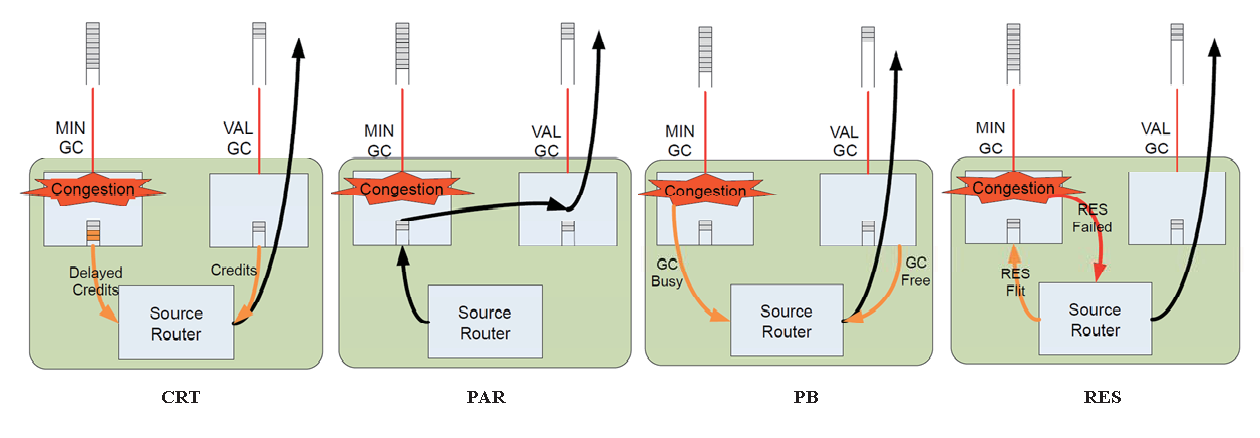
\includegraphics[width=.8\textwidth]{Visio-dragonfly_indirect.eps}
    \caption{Dragonfly结构间接自适应路由算法\upcite{indirect}}
       \label{dragonflyir}
\end{figure}

针对一些特定的通信负载,如最差通信负载,
Dragonfly结构中确定的两个超级节点频繁通信,
不仅会造成全局链路拥塞,还会同时造成本地链路拥塞。
如图\ref{dragonflytr}所示,
在采用了VAL的路由选择后仍然会造成同一个超级节点的
两个路由器因为要转发所连接全局链路传送来的报文导致两个路由器之间的本地链路拥塞。
%% FIXME 结合这个图,上面这句话说的似乎不太明确,我没看懂。
因此,研究者提出On-the-Fly 自适应路由算法(OFAR)\upcite{On-the-Fly}
来解决本地链路和全局链路的拥塞问题。
OFAR通过允许在超级节点内部进行本地链路的绕路,
有效避免了因为全局链路拥塞造成的本地链路的拥塞。
OFAR最长路径长度要达到8跳,如果采用VC隔离的方式避免死锁则至少需要6条VC。
OFAR最初采用的是基于气泡流量控制的哈密尔顿环作为逃逸子网,
OFAR-CM\upcite{OFAR-CM}则在OFAR 的基础上提出拥塞管理机制ECM和BCM,
这两种拥塞控制机制分别关注的是逃逸子网的拥塞情况和正常网络的拥塞情况,
该研究还提出采用树型逃逸子网和up-down路由算法。

\begin{figure}[htp]
  \centering
    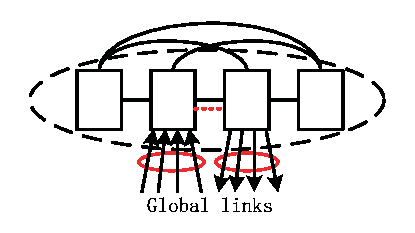
\includegraphics[width=.45\textwidth]{Visio-dragonfly_traffic.eps}
    \caption{Dragonfly结构中全局链路导致本地链路拥塞}
       \label{dragonflytr}
\end{figure}

路由算法中的死锁避免,有多种方法,大致可以分为三类:
一是设计无环路由,二是通过虚拟通道(VC)切换的方式避免死锁,
三是通过逃逸子网的方式避免死锁。
这其中,无环路由是最经济的方法,但是会因限制部分路径不能通行,降低网络吞吐率。
VC 切换的方法的优势是可以充分利用网络中的链路,
但是VC数量的增加给工艺和成本开销带来挑战。
逃逸子网使用一套独立的VC网络或者
物理网络执行一个没有环路的路由算法来避免整个网络的死锁,
相比前两种方法,逃逸子网可以算是一个折中的办法,
但是逃逸子网的使用频率影响网络性能。
RLM 和OLM算法\upcite{Rlmolm}的提出有效降低了OFAR对VC的需求。
RLM在超级节点内部采用转弯模型的方式避免死锁,即超级节点内部采用无环路由,
通过减少路径多样性降低VC数量。
OLM则是采用限制VC使用顺序的方式避免死锁,
利用VC降序作为逃逸路径,
在保证超级节点内的路径多样性的同时不额外增加VC数量。

除了考虑不同的通信负载和拓扑结构的特征,
也要考虑实际物理布局中缆线长短对路由算法决策的影响。
在\upcite{overcomefarend}中指出目前大多数
已有的工作都没有考虑远端延迟的影响,即下几跳后的网络拥塞和因路由器之间
较长链路延迟高引起的拥塞,实际上这些拥塞都只是暂时性的拥塞,
不会导致网络真正拥塞。
比如,较长的链路延迟会使得一些报文或者信用不能及时到达终点从而造成拥塞的假象。
因此,作者通过历史窗口的方法来避免这种假象影响自适应路由的决策
\upcite{overcomefarend}。

另外,是否能够合理分配缓冲区资源也是路由算法的性能的影响因素。
Gorgues等人\upcite{Achieving}提出在$k\textrm{-}ary$ $n\textrm{-}cube$结构的片上网络上,
通过报文标记的方法给报文均衡分配网络中的缓冲区资源并利用更少的资源来避免死锁。
具体设计是每个输入端口有2条VC,
每条VC被分配一个报文长度的缓冲区大小。
完全自适应路由算法通过通过一条逃逸路径来避免死锁。
每次路由决策都可能改变报文的标记,
如果报文的决策是按维序路由算法路由的话就被标记为安全报文。
否则,则被标记为不安全报文。
每个端口的两条VC中至少有一条VC里全是安全报文或者为空。
我们考虑将这种方法运用在片间网络上,不仅可以避免工艺上的挑战又能充分利用网络资源。

Head-of-Line Blocking(HoLB)问题也是影响路由算法性能的重要因素。
HoLB问题是指位于队列头的报文因为下一级拥塞不能前进阻挡了队列中其他报文前进。
相比确定性路由算法,即在源节点已经确定好报文传输路径,
自适应路由算法因为路由的灵活性会造成报文传输路径不唯一,
更容易造成HoLB问题\upcite{holbara}。
有研究组针对不同拓扑结构路由算法的HoLB问题提出了解决办法。
如在\upcite{holbara}中,针对直接网络的自适应路由算法,
利用有限的VC,将不同目的节点的报文分配到不同的VC中传输。
在\upcite{bbq}\upcite{DBBM}\upcite{iodet}中,
都使用类似的方法解决HoLB问题。
另外,提出上述方法的研究组也针对Dragonfly结构、Slim Fly结构
等典型新型高性能互连网络拓扑结构的路由算法提出了HoLB问题的解决方案
\upcite{holbdf}\upcite{holbsf}。
在FlexVC\upcite{flexvc}中则是提出一个缓冲区管理策略来降低网络HoLB问题,
具体方法就是在保证无死锁的前提下,
尽可能的增大VC可选择的范围。
如针对Slim Fly结构,如果采用最短路径路由算法,
网络中有3条VC的时候,报文就可以选择Opportunistic路径进行路由来降低HoLB问题。

\section{高性能互连网络拥塞控制机制}
拥塞控制机制与路由算法是影响高性能互连网络网络性能的重要因素。
自适应路由算法旨在解决网络中的链路拥塞问题,
而拥塞控制机制则是解决终端节点的超额订购。
当两者搭配使用才能更好的提升网络性能。
%% FIXME 把这句话从后面移到此处,是否使得后面CBCM的表述不清楚?

由于高性能互连网络具备无损的特性,即不会因为网络拥塞而丢包,
传统的拥塞控制机制,如TCP协议,就不适用于高性能互连网络。
高性能互连网络中经典的拥塞控制机制,
如Explicit Congestion Notification(ECN)拥塞控制机制,
是一种被动的拥塞控制机制,根据缓冲队列长度,
给报文打标签,到达目的节点后将拥塞信息通过ACK报文告诉源节点。
这种策略最大的缺点就是不能及时对拥塞作出反馈,响应速度慢。
在2012年的SC会议上,Jiang等人提出
Speculative Reservation Protocol (SRP)\upcite{srp}拥塞控制机制。
SRP是一种主动拥塞控制机制,
通过light-weight的终端预约机制以及投机报文传输机制有效缓解热点通信模式下的拥塞,
获得比ECN机制更高的吞吐率。
之后,该研究组在2013 年SC会议上提出
Channel Reservation Protocol(CRP)\upcite{crp}策略,
专门解决大规模无损网络通信中关键链路拥塞的问题。
因为考虑到成本和技术的限制,集群之间的链路都是供小于求,
如图\ref{crp}所示,如果热点H不能正常吸收负载则会造成
数据流Z拥塞在点A,进而产生拥塞树,
不仅影响集群0的数据流Y还影响集群1内要到达点H的数据流。
CRP通过预约关键链路的方法来解决瓶颈链路拥塞的问题。
在2015年的SC会议上,
该研究组针对ECN和SRP对small message终端拥塞反应速度慢和易造成
拥塞树等不足,
提出Small-Message SRP(SMSRP)和
Last-Hop Reservation Protocol (LHRP)两种策略\upcite{smsrp}。
相较于SRP策略,
SMSRP策略会在发送预约报文之前发送一些投机报文以免造成带宽浪费
以及因为预约产生的动荡。
LHRP相较于SRP和SMSRP策略的不同之处是在最后一跳交换机处根据终端的缓冲队列长度对
投机报文传输失败作出反馈。

\begin{figure}[htp]
  \centering
    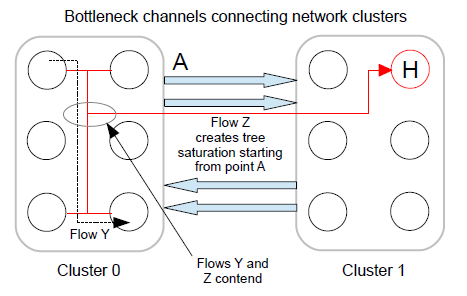
\includegraphics[width=.65\textwidth]{crp.png}
    \caption{集群间的拥塞树\upcite{crp}}
       \label{crp}
\end{figure}

除了上述基于预约的拥塞控制机制,Kim等人在2016年的MICRO会议上
提出一种新的拥塞管理策略Contention-based Congestion Management(CBCM)
\upcite{cbcm}。该研究指出,当网络中只采用自适应路由算法来提升网络性能的时候,
往往会造成拥塞扩散性能降低的情况。
CBCM的原理如图\ref{cbcm}所示,CBCM专门使用一条额外的VC分离终端拥塞的影响,
一旦发现终端拥塞,即终端接收到被标记的报文超过阈值,
则节流相应的源节点,且节流的报文在此额外的VC中采用最短路由算法,
从而避免因为自适应路由算法扩散拥塞。

\begin{figure}[htp]
  \centering
    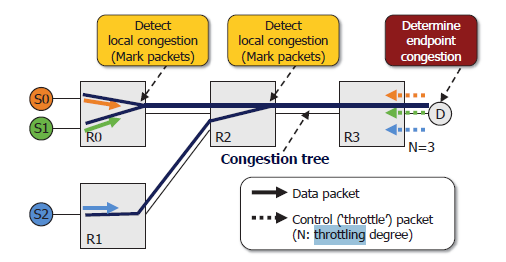
\includegraphics[width=.65\textwidth]{cbcm.png}
    \caption{Contention-based Congestion Management机制\upcite{cbcm}}
       \label{cbcm}
\end{figure}
%\section{模拟环境和性能测试平台}

\section{本章小结}
本章主要阐述了大规模低直径高性能互连网络的理论基础和相关研究。
主要综述了目前已提出的典型高性能互连网络的拓扑结构和典型路由算法、拥塞控制机制等内容。
%% 本文基于大规模低直径的特点开展高性能互连网络拓扑结构设计和路由算法的研究。



%%% Local Variables:
%%% mode: latex
%%% TeX-master: "../main"
%%% End:

\begin{ack}

四年半的博士时光匆匆而过,在论文即将完成之际,回首四年半来的学习、工作和生活,中间有过迷茫、有过痛苦、有过喜悦,但此刻充满我心中的是深深的感激之情,感谢那些给予
我关心和帮助的老师、同学和朋友,你们的关心与帮助不仅使我能够顺利完成博士学业,而且是我今后一生受用不尽的财富。言语已经不能完全表达我的感激之情,我需要在今后工作、生活中用行动来报答。但是我还是想在这里写下一些感激的文字,以表达我衷心的感恩之情!

感谢我的导师廖湘科研究员! 无论是学习、科研工作,还是生活中的大事小情,亦或做人处世,您都给了我无微不至的关怀和帮助。您勤奋严谨的治学态度、对科学问题的深邃洞察力、对学术方向的高瞻远瞩以及对新领域积极探索的精神,都是我不断成长的力量源泉,是我终生学习的榜样。您指导了我的人生之路,事业之路,是我用今后一生都报答不尽的。特别感谢我们的谢师母!谢师母是慈母,也是良师,是益友!您温暖的笑容,让我们感受到了慈母般的关怀!

感谢董德尊研究员!您渊博的学识、敏锐的洞察力、勤奋进取的科研精神、严谨的治学态度以及平易近人、待人友善的生活作风,无时无刻不在熏陶和感染着我,并将让我终身受益。每当碰到困难与问题向您求教时,总能获得您宝贵的建议和解决问题的思路,让我受益匪浅。您带我走进了高性能互连网络这一研究领域,认识到这一领域在国际上的发展趋势。在您的指导下,完成了多篇学术论文。这些论文的选题、研究以及最后的撰写,都凝结了您的心血。您还让我接触到了多位国际知名学者,开阔了我的视野。感谢嫂子姬少丽!嫂子对董师兄工作的支持和理解,让我们充满敬意!

感谢Jose Duato教授!在我访学西班牙瓦伦西亚理工大学期间以及通过邮件讨论给我在课题上提供了很大的帮助和宝贵的意见,并在悉心指导下,完成了相关问题学术论文的撰写。

感谢我所在的教研室的领导和老师们!你们为我提供了良好的学习科研环境,并给予我大量具有创造性和启发性的指导!

感谢杨沙洲师兄和李姗姗师姐!硕士入学,是他们开启了我的学术科研之旅,是他们治学严谨的科研精神感染了我!

感谢互连研究团队的成员!吴际、保金桢、李存禄、柴燕涛、杨明英、方磊、李彬、娄辉、朱成阳、杨文祥、徐叶茂、师凯、杜记伟、张庆安、张敏、赵静月、邹祥喜、祝雅正、张凡、吴君楠、孙凯旋、黄山、朱佳平、杨天野、魏子昊、吴克、金康、周择嘉、张鑫、白洋,和你们一起学习、奋斗,营造了和谐、团结、奋进的实验室氛围,和大家一起的奋斗的时光将成为美好的回忆!也要谢谢从事其它研究工作的师兄弟们!他们是鲁晓佩、刘晓东、郑思、林彬、朱浩、张菁、郭勇、黄訸、任静、范小康、申彤、张峰、徐尔茨、崔英博、贾周阳、周书林、顾祥、徐向阳、郦旺、张晓雨、李云峰、刘晋宇、池书琪、王腾、张元良、何浩辰。

感谢多年来一直支持和陪伴的好友和同学!感谢206大家庭王倩、丰瑶、杨静、史乔给予我的温暖!感谢郭辉、陈辰、陆华俊一起游历祖国大江南北!感谢宋省身、陈洪义一起探索美食运动和时事!感谢曾皓、陈呈、高涛一起探讨人生学术和理想!感谢邻居李豪和岑阳夫妇!感谢14级2班的全体成员!感谢组委会的兄弟姐妹们!

感谢博士生队的队领导们对我的关怀和帮助,他们默默践行着为学员创造良好环境的承诺,为我们的科研和生活提供了稳固的保障。
感谢本文及相关小论文的所有评审老师!你们的评审意见为论文的改进与完善提供了很大的帮助!

感谢我的父母其他亲人! 没有你们的支持、理解和鼓励就没有我的一切。

感谢我的爱人苏醒,相知相遇一路走来,非常幸运一起携手经历博士生涯。愿我们
共同努力奋斗,一起迎创新的未来!

最后,再次诚挚地感谢所有给予我关心与帮助的以及未能列出名字的领导、老师、亲人和朋友们,感谢你们!



\end{ack}


%</thesis>
%    \end{macrocode}
%
% 在\LaTeX{}下管理参考文献将极其方便,建议使用Jabref生成条目,
% 用\verb|\cite|(其中\verb|upcite|是上标索引)索引即可。
% \verb|refs.bib|是你的参考文献名。
%    \begin{macrocode}
%<*thesis>
\cleardoublepage
\phantomsection
\addcontentsline{toc}{chapter}{参考文献}
\bibliographystyle{bstutf8}
\bibliography{ref/refs}

\begin{resume}

  \section*{发表的学术论文} % 发表的和录用的合在一起

  \begin{enumerate}[{[}1{]}]
  \addtolength{\itemsep}{-.36\baselineskip}%缩小条目之间的间距,下面类似
  \item Fei Lei, Dezun Dong, Xiangke Liao, Xing Su, and Cunlu Li. Galaxyfly: A Novel Family of Flexible-Radix Low-Diameter Topologies for Large-Scales Interconnection Networks. in Proceedings of the 2016 International Conference on Supercomputing(ICS), 2016, pp. 24:1–24:12.(EI检索号:20163002626759,CCF B类会议)
  \item Fei Lei, Dezun Dong, Xiangke Liao. An Efficient Label Routing on High-Radix Interconnection Networks. in Proceedings of the 2017 International Conterence on Parallel and Distributed Systems (ICPADS), 2017, pp.596-603.(EI检索号:20182405316608,CCF C类会议)
   \item Fei Lei, Dezun Dong, and Xiangke Liao. Exploring the Galaxyfly Family to Build Flexible-Scale Interconnection Networks. (已投稿至 Transactions on Computers (TC),CCF A类期刊).
   \item Fei Lei, Dezun Dong, Xiangke Liao, and Jose Duato. Exploring the Galaxyfly Family to Build Flexible-Scale Interconnection Networks. (已投稿至 ACM Transactions on Architecture and Code Optimization(TACO),CCF B类期刊).
  \item 雷斐,董德尊,庞征斌,廖湘科,杨明英. Paleyfly:一种可扩展的高速互连网络拓扑结构[J].计算机研究与发展, 2015. 52(6):1329-1340.(EI检索号:20152901043559)
  \item 雷斐, 董德尊, 廖湘科. SuperStar:一种可扩展高阶互连拓扑结构[J]. 计算机工程与科学, 2014. 36(6):39-46 .
  \item 雷斐,董德尊,柴燕涛,王克非,李存禄. 高阶互连网络拓扑结构性能分析与研究[J]. 计算机工程与科学, 2013. 35(11):111-118 .
  \item 杨明英,雷斐,董德尊,沈胜宇,庞征斌.一种新型混合互连网络拓扑结构的分析与优化[J].计算机工程与科学, 2014. 36(12):2400-2409.
  \item Cunlu Li, Dezun Dong, Xiangke Liao, Ji Wu, Fei Lei. RoB-Router: Low Latency Network-on-Chip Router Microarchitecture Using Reorder Buffer. in Proceedings of the 2016 IEEE Hot Interconnects (HOTI), 2016, pp.68-75. (EI检索,检索号:20170503305832)
  \item	Cunlu Li, Dezun Dong, Xiangke Liao, Fei Lei, Ji Wu. CCAS: Contention and congestion aware switch allocation for network-on-chips. in Proceedings of the 34th IEEE International Conference on Computer Design (ICCD), 2016, pp.444-447. (EI检索,检索号:20165203166084)
  \item 李存禄, 董德尊, 吴际, 雷斐, 王克非, 廖湘科. 低延迟路由器中高效开关分配机制的实现与评测. [J]. 湖南大学学报(自然版), 2015. 42(4): 78-84. (EI检索,检索号:20151900831996)
  \item 杨文祥, 董德尊, 李存禄, 雷斐, 孙凯旋, 吴际. 一种多级无缓存高阶路由器的设计与实现. [J]. 计算机工程与科学, 2017, 39(2):245-251.
  \item 杨文祥, 董德尊, 李存禄, 雷斐, 吴际, 孙凯旋. 高阶路由器结构研究综述. [J]. 计算机工程与科学, 2016, 38(8):1517-1523.
  \end{enumerate}

  \section*{研究成果} % 有就写,没有就删除
  \begin{enumerate}[{[}1{]}]
  \addtolength{\itemsep}{-.36\baselineskip}%
  \item 董德尊, 保金桢, 赵宝康等. 一种支持大规模、全光互连的光交换机: 中国,
     CN105681932A (中国专利公开号).
  \end{enumerate}


\section*{参与的科研工作}

  \begin{enumerate}[{[}1{]}]
  \addtolength{\itemsep}{-.36\baselineskip}%
  \item 国防预研项目:大规模互连网络模拟仿真技术
  \item 国家重点研发计划项目:基于数据流的大数据分析系统
  \item 国家“863”计划重大项目:天河新一代高性能计算机系统研制
  \item 国家重点研发计划项目:百亿亿次E级超算原型系统研制
  \end{enumerate}
\end{resume}

%</thesis>
%    \end{macrocode}
%
%<thesis>% 最后,需要的话还要生成附录,全文随之结束。
%    \begin{macrocode}
%<*thesis>
\appendix
\backmatter
\input{data/appendix01}

\end{document}
%</thesis>
%    \end{macrocode}
%
% 当然还有一些收尾工作,校验审阅自不必说。接下来你需要:修改论文中英文日期,
% 生成盲评,生成明(盲)评A3封面。
%
% {\color{blue}Happy \TeX{}ing! 欢迎提各式各样的意见!}
%
% \newpage\relax%
%
% \StopEventually{\PrintChanges}
% \clearpage
%
% \section{实现细节}
% 我们首先介绍文档模板的基本信息以及宏包和配置,
% 然后依照国防科学技术大学论文模板的书写规范一节一节的介绍实现步骤。
%
% \changes{v1.2}{2009/09/28}{添加了A3封面制作}
%
% \subsection{基本信息}
%    \begin{macrocode}
%<cls>\NeedsTeXFormat{LaTeX2e}[1999/12/01]
%<cls>\ProvidesClass{nudtpaper}
%<cfg>\ProvidesFile{nudtpaper.cfg}
%<cls|cfg>[2011/07/17 v2.2 NUDT paper template]
%    \end{macrocode}
%
% \subsection{宏包配置}
%
%<*cls>
%
%\changes{v0.99}{2009/08/17}{add package options}
% 当前的宏包选项在之前已经介绍了,下面是实现步骤,就是几个\verb|if|。
%\changes{v1.6}{2009/12/01}{添加单独的单双面控制}
%\changes{v2.0}{2010/11/09}{添加盲评控制}
%
%    \begin{macrocode}
\newif\ifismaster\ismastertrue
\newif\ifisttf\isttffalse
\newif\ifisfz\isfzfalse
\newif\ifisotf\isotffalse
\DeclareOption{master}{\ismastertrue}
\DeclareOption{doctor}{\ismasterfalse}
\newif\ifisanon\isanonfalse
\DeclareOption{anon}{\isanontrue}
\newif\ifistwoside\istwosidefalse
\DeclareOption{twoside}{\istwosidetrue}
\DeclareOption{ttf}{\isttftrue}
\DeclareOption{fz}{\isfztrue}
\DeclareOption{otf}{\isotftrue}
\newif\ifisvista\isvistafalse
\DeclareOption{vista}{\isvistatrue}
\DeclareOption*{\PackageWarning{nudtpaper}{Unknown Option '\CurrentOption'}}
\ProcessOptions\relax
%    \end{macrocode}
%
% 首先调用在文档类书写中需要的过程控制语句,在计算一些\verb|length|时要用到
%    \begin{macrocode}
\RequirePackage{ifthen,calc}
%    \end{macrocode}
%
% 接着我们导入文本类,该模板基于标准的书籍模板book,其默认格式为单面打印。
% 博士论文如需双面打印,必须指定\verb|twoside|选项。双开的含义是章节总是
% 起在右手边,左手空白页为完全的空白页,不包含页眉页脚。
%
% \changes{v1.6}{2009/12/01}{修改开关选项}
%
%    \begin{macrocode}
\ifistwoside
  \LoadClass[a4paper,12pt,openright,twoside]{book}
\else
  \LoadClass[a4paper,12pt,openany]{book}
\fi
%    \end{macrocode}
%
% 我们直接用\textsf{geometry}宏包进行页面边距的设定,调用titlesec设定标题以及页眉页脚,
% 用\textsf{titletoc}设定目录格式。需要改动的可以参考这三个宏包的说明文档。
%
%    \begin{macrocode}
\RequirePackage[includeheadfoot]{geometry}
\RequirePackage[center,pagestyles]{titlesec}
\RequirePackage{titletoc}
%    \end{macrocode}
%
% 文档中另外重要的两个部分是表格和图片。
% 首先来看图片:\textsf{graphicx}宏包是必不可少的,
% 并排图形。\textsf{subfigure} 已经不再推荐,用新的 \textsf{subfig}。
% 加入 \verb|config| 选项
% 以便兼容 \textsf{subfigure} 的命令。浮动图形和表格标题样式。\textsf{caption2} 已经不
% 推荐使用,采用新的 \textsf{caption}。它会自动被 \textsf{subfig} 装载进来。所以可以在
% 后面使用 \textbf{captionsetup} 命令,宏包\textsf{float}的作用是可以用H命令,
% 将浮动对象强制放在这里(副作用是版面可能不好):
%
%    \begin{macrocode}
\RequirePackage{graphicx}
\RequirePackage[config]{subfig}
\RequirePackage{float}
%    \end{macrocode}
%
% 再来看表格:我们采用\textsf{longtable}来处理长的表格,还需要\textsf{array}包;
% 标准的论文需要表格为三线表,这里引用\textsf{booktabs}宏包来处理,
% 这样,我们就可以简单的使用\verb|\toprule|,\verb|\midrule|,\verb|bottomrulle|
% 这样的命令;
% 为了在表格中支持跨行,需要引入\textsf{multirow}包,\textsf{tabularx}的作用是为了使用
% 固定宽度的表格,\textsf{slashbox}可以让我们在表格中使用反斜线:
%    \begin{macrocode}
\RequirePackage{array}
\RequirePackage{longtable}
\RequirePackage{booktabs}
\RequirePackage{multirow}
\RequirePackage{tabularx}
\RequirePackage{slashbox}
%    \end{macrocode}
% 表格和图片的例子可以搜索C\TeX{}论坛或者看示例文件。
%
% 引入\textsf{paralist}来达到比较好看的列表环境
%    \begin{macrocode}
\RequirePackage[neverdecrease]{paralist}
%    \end{macrocode}
%
% 文档中还需要一定的色彩控制和字体控制
%    \begin{macrocode}
\RequirePackage{xcolor}
%    \end{macrocode}
%
% 为了排出漂亮的数学公式,\textsf{amsmath}包是必不可少的,
% 需要注意的是,新版本的论文模板仍旧使用\textsf{txfonts}宏包,
% 为了支持希腊正体字母,需要调用\verb|upgreek.sty|,使用方法是\verb|\up<greek>|。
% 注意到这个宏包前面加上了\verb|Symbolsmallscale|选项,这是为了配合
% \verb|txfonts|希腊字体的大小而设定的。如果用户不满意这个宏包的积分号
% 等符号,倾向与使用传统的\LaTeX{}风格的数学符号,那么可以使用
% \textsf{mathptmx}宏包,但要把\verb|upgreek|的选项改为\verb|Symbol|,要不然
% 正体希腊字母要显得小一点哦。
% 而大写斜体希腊字母(变量)可以通过\textsf{amsmath}的\verb|\var<Greek>|得到。
% 当然,对于希腊字母的加粗推荐使用\verb|bm|宏包,一般变量的加粗那就使用
% \verb|\mathbf|吧!
% \changes{v2.0}{2010/11/09}{去掉fontspec,传递no-math到xeCJK,加入bm宏包}
% \changes{v2.2}{2011/07/16}{去掉txfonts宏包,使用lm字体,添加svgreek.sty}
% \changes{v2.2}{2011/07/16}{修改,仍旧使用upgreek, mathptmx, bm组合}
% \changes{v2.2}{2011/09/25}{修改,使用upgreek, txfonts, bm组合}
% \changes{v2.2}{2012/11/28}{给用户提供额外的选项,还是mtpro比较漂亮}
% \changes{v2.3}{2013/12/27}{调整数学字体,加入mtpro使用说明,并且仿照IEEE模板,修改displaypenalty}
%    \begin{macrocode}
\RequirePackage{amsmath,amssymb}
\RequirePackage{txfonts}
\RequirePackage[Symbolsmallscale]{upgreek}
%\RequirePackage{amsmath}
%\RequirePackage[amsbb,eufrak,compatiblegreek,subscriptcorrection,nofontinfo]{mtpro2}
\interdisplaylinepenalty=2500
\RequirePackage{bm}
\RequirePackage[T1]{fontenc}
\RequirePackage[amsmath,thmmarks,hyperref]{ntheorem}
%    \end{macrocode}
% 需要注意的是,如果用户有\verb|mtpro2|包,还是强烈建议使用这个的,因为数学公式
% 在这个包下显得特别的美观。虽然下载和安装不属于这篇使用说明的范畴,但是,上面的注释部分
% 可以给大家如何使用的一个简单的例子。当你安装好\verb|mtpro2|之后,主要取消注释,并且将
% 上面的三个包注释掉即可。
%
% 本文档类直接采用\XeTeX{}引擎,方便了字体配置以及编译,
% 这里需要调用\textsf{XeCJK}宏包,no--math的作用是不改变先前数学宏包设定的数学字体。
% 同时采用\textsf{indentfirst}宏包管理文字的缩进:
% \changes{v1.8}{2010/10/15}{修改了默认的xeCJK的选项,为了兼容旧的xeCJK版本,normalindentfirst选项暂不使用,而是在后面添加indentfirst包}
% \changes{v2.0}{2010/11/10}{传递no-math给xeCJK里面的fontspec宏包}
% \changes{v2.2}{2011/07/03}{移除CJKtextspace, CJKmathspace, CJKnumber选项}
%
%    \begin{macrocode}
\RequirePackage[CJKnumber,CJKchecksingle,no-math]{xeCJK}
\RequirePackage{indentfirst}
%    \end{macrocode}
%
% 另外一个关键部分是文献索引,包括书签以及参考文献的索引,记得\textsf{hyperref}配合
% \XeTeX{}使用时暂不能开启Unicode选项,新的发行版已经移除\textsf{hypernat}包。另外还要注意,你最终的打印版肯定
% 不希望有花花绿绿的链接,对吧?那就把下面那行\verb|hyperref|注释掉就行了。
% \changes{v2.1}{2010/12/29}{移除hypernat包}
% \changes{v2.2}{2011/07/17}{移除hyperref的CJKbookmarks旋向}
% \changes{v2.3}{2013/12/27}{加入色彩版hyperref}
%    \begin{macrocode}
\RequirePackage[numbers,sort&compress,square]{natbib}
\RequirePackage[colorlinks=true,linkcolor=blue,citecolor=red,pdfborder=0 1 1]{hyperref}
%\RequirePackage[pdfborder=0 0 1]{hyperref}
%    \end{macrocode}
%</cls>
%
%\subsection{基础配置}
% 本章主要介绍模板中用到的基本的元素和定义,现在包括两部分: 字体,字号和字体命令
%
%\subsubsection{字体定义}
% 我们首先来处理\TeX{}中最令人棘手的字体问题,
% 在使用\textsf{XeCJK}包之后,配置和选择很容易,
% 预先设定好一些字体命令是为了后面方便的更改文本字体的需要。
% 首先我们开启\TeX{}连字符:
%    \begin{macrocode}
%<*cls>
\defaultfontfeatures{Mapping=tex-text}
%</cls>
%    \end{macrocode}
%
% 之后用\textsc{XeCJK}包提供的命令设定字体,用户可以选择使用TTF还是OTF字体,
% Adobe的OpenType字体在排版上更具备优势,文档显示锐利,推荐使用。
% 另外在这一个新版本中,我们推荐用户也可以使用方正的字体,只要使用\verb|FZ|选项即可。
% 中注释掉相关的字体就可以。方正字体的有点是标点符号的位置无需修正,且字体之间配合很好。
% \verb|setcharclass|的作用是纠正xunicode、xeCJK的一些设定:
%
% \changes{v0.99}{2009/08/17}{add options TTF and OTF}
% \changes{v0.993}{2009/08/25}{加入VISTA用户选项}
% \changes{v1.9}{2010/10/28}{定义一个cusong字体,使用的是中宋}
% \changes{v2.3}{2013/12/27}{用户可以考虑使用方正字体,加入FZ选项}
%
%    \begin{macrocode}
%<*cls>
\xeCJKsetcharclass{"0}{"2E7F}{0}
\xeCJKsetcharclass{"2E80}{"FFFF}{1}
\newcommand\installTTF{%
  \setmainfont{Times New Roman}
  \setsansfont{Arial}
  \setmonofont{Courier New}
  \ifisvista
    \setCJKmainfont[BoldFont={SimHei},ItalicFont={KaiTi}]{SimSun}
    \setCJKmonofont{KaiTi} % Pluto use LiSu Thu use Kaiti, orig is SimSun
    \setCJKfamilyfont{fs}{FangSong}
    \setCJKfamilyfont{kai}{KaiTi}
  \else
    \setCJKmainfont[BoldFont={SimHei},ItalicFont={KaiTi_GB2312}]{SimSun}
    \setCJKmonofont{KaiTi_GB2312} % Pluto use LiSu Thu use Kaiti, orig is SimSun
    \setCJKfamilyfont{fs}{FangSong_GB2312}
    \setCJKfamilyfont{kai}{KaiTi_GB2312}
  \fi
  \setCJKsansfont{SimHei}
  \setCJKfamilyfont{song}{SimSun}
  \setCJKfamilyfont{hei}{SimHei}
  \setCJKfamilyfont{li}{LiSu}
  \setCJKfamilyfont{you}{YouYuan}
  \setCJKfamilyfont{cusong}{STZhongsong}
}
\newcommand\installOTF{%
  \setmainfont{Times New Roman} % could be changed to "Times New Roman PS Std" !!
  \setsansfont{Arial}
  \setmonofont{Courier New}
  \setCJKmainfont[BoldFont={Adobe Heiti Std},ItalicFont={Adobe Kaiti Std}]{Adobe Song Std}
  \setCJKsansfont{Adobe Heiti Std}
  \setCJKmonofont{Adobe Kaiti Std}
  \setCJKfamilyfont{song}{Adobe Song Std}
  \setCJKfamilyfont{hei}{Adobe Heiti Std}
  \setCJKfamilyfont{fs}{Adobe Fangsong Std}
  \setCJKfamilyfont{kai}{Adobe Kaiti Std}
  \setCJKfamilyfont{li}{Adobe Kaiti Std}
  \setCJKfamilyfont{you}{Adobe Kaiti Std}
  \setCJKfamilyfont{cusong}{STZhongsong}
}
\newcommand\installFZ{%
  \setmainfont{Times New Roman} % could be changed to "Times New Roman PS Std" !!
  \setsansfont{Arial}
  \setmonofont{Courier New}
  \setCJKmainfont[BoldFont={FZHei-B01},ItalicFont={FZKai-Z03}]{FZShuSong_GB18030-Z01}
  \setCJKsansfont{FZHei-B01} % Hei
  \setCJKmonofont{FZKai-Z03} % Kai
  \setCJKfamilyfont{song}{FZShuSong_GB18030-Z01}
  \setCJKfamilyfont{hei}{FZHei-B01}
  \setCJKfamilyfont{fs}{FZKai-Z03} % Kai
  \setCJKfamilyfont{kai}{FZKai-Z03} % Kai
  \setCJKfamilyfont{li}{FZKai-Z03} % Kai
  \setCJKfamilyfont{you}{FZKai-Z03} % Kai
  \setCJKfamilyfont{cusong}{FZXiaoBiaoSong-B05} % 小标宋
}
\newcommand{\cusong}{\CJKfamily{cusong}} % 中宋作为加粗宋体
%</cls>
%    \end{macrocode}
%
% \changes{v1.6}{2009/12/01}{替换OTF英文字体为标准Windows自带字体}
% \changes{v2.3}{2013/12/27}{添加FZ字体选项}
% 之后我们根据你的设定决定安装什么字体:
%
%    \begin{macrocode}
%<*cls>
\ifisttf
  \installTTF
\else
  \ifisfz
    \installFZ
  \else
    \installOTF
  \fi
\fi
%</cls>
%    \end{macrocode}
%
% 选定好字体之后,就是设定字体别名,这样我们就可以在文档的其他部分直接使用较短的命令来
% 指定特定的字体了:
%
%    \begin{macrocode}
%<*cls>
\newcommand{\song}{\CJKfamily{song}}    % 宋体
\newcommand{\fs}{\CJKfamily{fs}}        % 仿宋体
\newcommand{\kai}{\CJKfamily{kai}}      % 楷体
\newcommand{\hei}{\CJKfamily{hei}}      % 黑体
\newcommand{\li}{\CJKfamily{li}}        % 隶书
\newcommand{\you}{\CJKfamily{you}}      % 幼圆
\def\songti{\song}
\def\fangsong{\fs}
\def\kaishu{\kai}
\def\heiti{\hei}
\def\lishu{\li}
\def\youyuan{\you}
%</cls>
%    \end{macrocode}
%
% \subsubsection{字号定义}
%下面就是定义字号大小,这一部分我们有两个参考,其一是:
%
% \begin{verbatim}
% 参考科学出版社编写的《著译编辑手册》(1994年)
% 七号      5.25pt       1.845mm
% 六号      7.875pt      2.768mm
% 小五      9pt          3.163mm
% 五号      10.5pt       3.69mm
% 小四      12pt         4.2175mm
% 四号      13.75pt      4.83mm
% 三号      15.75pt      5.53mm
% 二号      21pt         7.38mm
% 一号      27.5pt       9.48mm
% 小初      36pt         12.65mm
% 初号      42pt         14.76mm
%
% 这里的 pt 对应的是 1/72.27 inch,也就是 TeX 中的标准 pt
% \end{verbatim}
%
% 另外一个来自WORD中的设定:
% \begin{verbatim}
% 初号 = 42bp = 14.82mm = 42.1575pt
% 小初 = 36bp = 12.70mm = 36.135 pt
% 一号 = 26bp = 9.17mm = 26.0975pt
% 小一 = 24bp = 8.47mm = 24.09pt
% 二号 = 22bp = 7.76mm = 22.0825pt
% 小二 = 18bp = 6.35mm = 18.0675pt
% 三号 = 16bp = 5.64mm = 16.06pt
% 小三 = 15bp = 5.29mm = 15.05625pt
% 四号 = 14bp = 4.94mm = 14.0525pt
% 小四 = 12bp = 4.23mm = 12.045pt
% 五号 = 10.5bp = 3.70mm = 10.59375pt
% 小五 = 9bp = 3.18mm = 9.03375pt
% 六号 = 7.5bp = 2.56mm
% 小六 = 6.5bp = 2.29mm
% 七号 = 5.5bp = 1.94mm
% 八号 = 5bp = 1.76mm
%
% 1bp = 72.27/72 pt
% \end{verbatim}
%
% 我们采用习惯的字号设定方法(也就是WORD中的设定),首先编写字体设置命令:
%
%\begin{macro}{\choosefont}
% 我们可以使用 |\choosefont| 来选择字体, 字体设定这些大多是从清华的模板拷过来的。
%
%    \begin{macrocode}
%<*cls>
\newlength\thu@linespace
\newcommand{\thu@choosefont}[2]{%
    \setlength{\thu@linespace}{#2*\real{#1}}%
    \fontsize{#2}{\thu@linespace}\selectfont}
\def\thu@define@fontsize#1#2{%
    \expandafter\newcommand\csname #1\endcsname[1][\baselinestretch]{%
    \thu@choosefont{##1}{#2}}}
%</cls>
%    \end{macrocode}
%\end{macro}
%
%设定具体的字体大小:
%
%    \begin{macrocode}
%<*cls>
\thu@define@fontsize{chuhao}{42bp}
\thu@define@fontsize{xiaochu}{36bp}
\thu@define@fontsize{yihao}{26bp}
\thu@define@fontsize{xiaoyi}{24bp}
\thu@define@fontsize{erhao}{22bp}
\thu@define@fontsize{xiaoer}{18bp}
\thu@define@fontsize{sanhao}{16bp}
\thu@define@fontsize{xiaosan}{15bp}
\thu@define@fontsize{sihao}{14bp}
\thu@define@fontsize{banxiaosi}{13bp}
\thu@define@fontsize{xiaosi}{12bp}
\thu@define@fontsize{dawu}{11bp}
\thu@define@fontsize{wuhao}{10.5bp}
\thu@define@fontsize{xiaowu}{9bp}
\thu@define@fontsize{liuhao}{7.5bp}
\thu@define@fontsize{xiaoliu}{6.5bp}
\thu@define@fontsize{qihao}{5.5bp}
\thu@define@fontsize{bahao}{5bp}
%</cls>
%    \end{macrocode}
%
%\subsubsection{自定命令}
% 有一些常量,测试,自定义的命令等都放在这里,待到论文逐渐完善之后再做定夺,
% 当然用户自己的命令也可以在此添加,事实上如果natbib传递的是superscript,
% \verb|cite|命令默认就成了上标了。这里不加入这个选项,而是单独编写一个命令:
%
%    \begin{macrocode}
%<*cls>
\newcommand{\upcite}[1]{\textsuperscript{\cite{#1}}} % 上标形式引用
\newcommand{\china}{中华人民共和国}
\def\nudtpaper{\textsc{Nudt}\textsc{Paper}}
\newcommand{\pozhehao}{\kern0.3ex\rule[0.8ex]{2em}{0.1ex}\kern0.3ex}
%</cls>
%    \end{macrocode}
%
%\subsubsection{中文元素}
%
% 默认的页面元素的英文名,诸如Contents为目录,Abstract为摘要等,
% 我们首先将他们一一中文化:
% \changes{v0.992}{2009/08/19}{修改图表编号格式}
% \changes{v1.3}{2009/10/14}{修改图目录和表目录}
%
%    \begin{macrocode}
%<*cls>
\renewcommand\contentsname{目\hspace{1em}录}
\renewcommand\listfigurename{图\hspace{1em}目\hspace{1em}录}
\renewcommand\listtablename{表\hspace{1em}目\hspace{1em}录}
\newcommand\listequationname{公式索引}
\newcommand\equationname{公式}
\renewcommand\bibname{参考文献}
\renewcommand\indexname{索引}
\renewcommand\figurename{图}
\renewcommand\tablename{表}
\renewcommand\appendixname{附录}
\def\CJK@today{\CJKdigits{\the\year} 年 \CJKnumber{\the\month} 月}
\newcommand\zhtoday{\CJK@today}
\newcommand\entoday{\today{}}
%</cls>
%    \end{macrocode}
%
% 好,下面就开始按照论文模板要求进行排版!
%
%\subsection{编写要求}
% 学校规定,论文需采用白色纸双面打印。
% 学位论文用A4($210mm\times{}297mm$)标准大小的白纸,
% 在打字或印刷时,要求纸的四周留足空白边缘,以便装订、复制和读者批注。
% 每一面的上方(天头)和下方(地角)分别留边25mm,左侧(订口)
% 和右侧(切口)分别留边30mm,页眉与页脚分别为23mm。
%
% 实现起来很简单,只要调用\textsf{geometry}的版面控制命令即可,
% 方法为先把word模板转化为PDF,
% 用Adobe的裁剪功能查看页边距,进行微调,直到比对正确为止,设定如下:
%
% \changes{v0.991}{2009/08/18}{modify bottom skip}
% \changes{v1.1}{2009/09/26}{修改footskip容限以及bottom的值,为了容下longtab的''下一页''}
% \changes{v1.4}{2009/10/28}{减小页眉skip 1mm,用word叠印}
% \changes{v1.4}{2009/10/30}{增大页眉sep .5mm,用word叠印}
%
%    \begin{macrocode}
%<*cls>
\geometry{top=21mm,bottom=25.5mm,left=30mm,right=30mm}
\geometry{headheight=9mm,headsep=1mm,footskip=9mm}
%</cls>
%    \end{macrocode}
%
%\subsection{页眉页脚}
%
% 我们采用titlesec进行页面配置。
% 页面中的主要元素有Chapter,Section,Subsection等元素的外观,
% 位置,颜色字体等,页面元素还包括页眉页脚。这种方法配置简便,易管理。
% 国防科大的论文需要在页眉处画两根横线,我们通过下面的命令实现:
%
%\begin{macro}{\setheadrule}
% 这个命令属于更改\textsf{titlesec}中的一个画页眉的命令,稍加调整:
% \changes{v0.991}{2009/08/18}{modify headrull, s.t. all geometry match}
% \changes{v1.9}{2010/10/28}{去掉headsep,修改headrule,在sethead后添加raisebox}
%
%    \begin{macrocode}
%<*cls>
\renewcommand\setheadrule[1]{%
  \ifdim#1=\z@
    \let\makeheadrule\@empty
  \else
    \def\makeheadrule{%
    \makebox[0pt][l]{\rule[.2\baselineskip]{\linewidth}{1.5pt}}%
    \rule{\linewidth}{1.5pt}}%
  \fi}
%</cls>
%    \end{macrocode}
%\end{macro}
%
% 由于Chapter第一页默认是\verb|plain|页面格式,
% 章节的其余部分是在Matter中设定的页面格式,为了简单起见,
% 我们就直接更改\verb|plain|页面设置,
% 要求为5号宋体居中放置,画页眉页脚,页脚为1磅黑线
%
% \changes{v0.992}{2009/08/20}{renewpagestyle里面前导的空格可能导致clearpage生成新的一页,将空格去掉}
% \changes{v0.993}{2009/08/26}{修改标题,博士硕士对应不同的页眉}
%
%    \begin{macrocode}
%<*cls>
\renewpagestyle{plain}{
\sethead{}{\raisebox{.65\baselineskip}{\songti \wuhao \ifisanon{~}\else{国防科学技术大学研究生院\@optionpaperclass{}学位论文}\fi}}{}%
\setfoot{}{{\songti \wuhao 第~\thepage~页}}{}%
\headrule%
\footrule%
}
\setfootrule{1bp}
%</cls>
%    \end{macrocode}
%
%\subsection{编写格式}
%
% 当页面设置好之后,就是在论文的不同部分分别调用,一般来说论文类的书籍
% 分为三个matter,为前言区(前置部分),正文区(主体),后文区(附录),
% 在国防科大论文书写要求中,
% 需要将摘要单独进行页码编号,其编号为小写罗马字母,为此,
% 可以将摘要单独设定为一个matter,
% 名叫就叫做MidMatter,称作摘要区。每个Matter我们都一一介绍。
%
% 首先看前置部分,主要包括封面,目录,摘要等,实现为:
%
%    \begin{macrocode}
%<*cls>
\renewcommand\frontmatter{%
    \if@openright\cleardoublepage\else\clearpage\fi
    \@mainmatterfalse
    \pagenumbering{Roman}
    \pagestyle{plain}}
\newcommand\midmatter{%
    \if@openright\cleardoublepage\else\clearpage\fi
    \@mainmatterfalse
    \pagenumbering{roman}
    \pagestyle{plain}}
%</cls>
%    \end{macrocode}
%
% 之后为文章的正文区,采用阿拉伯数字编页码:
%
%    \begin{macrocode}
%<*cls>
\renewcommand\mainmatter{%
    \if@openright\cleardoublepage\else\clearpage\fi
    \@mainmattertrue
    \pagenumbering{arabic}
    \pagestyle{plain}}
%</cls>
%    \end{macrocode}
%
% 最后是附录部分,由于他的章节标题与正文中不一样(不是第几章,而是附录几),
% 我们需要单独设定:
%
%    \begin{macrocode}
%<*cls>
\renewcommand\backmatter{%
    \if@openright\cleardoublepage\else\clearpage\fi
    \titleformat{\chapter}{\filcenter \heiti \sanhao}{附录\,\thechapter\,}{1em}{}
    \titlecontents{chapter}[0pt]{\vspace{0.25\baselineskip} \heiti \xiaosi[1.25]}
      {附录\,\thecontentslabel\quad}{}
      {\hspace{.5em}\titlerule*{.}\contentspage}
    \@mainmattertrue
    \pagestyle{plain}}
%</cls>
%    \end{macrocode}
%
% 我们重新定义\verb|cleardoublepage|,使得生成完全的空白页,页面模式为\verb|empty|
%    \begin{macrocode}
%<*cls>
\renewcommand\cleardoublepage{\clearpage\if@openright \ifodd\c@page\else
  \newpage{}
  \thispagestyle{empty}
  \vspace*{\fill}
  \begin{center}
  \end{center}
  \vspace*{\fill}
  \clearpage\fi\fi%
}
%</cls>
%    \end{macrocode}
%
%\subsubsection{前置目录}
% 前置部分的封面在后面详细介绍。首先看目录,要求为:
% 目次页由论文的章、节、条、项、附录等的序号、名称和页码组成,
% 另页排在序之后。目次页标注学位论文的前三级目录。
% 标题统一用“目录”,黑体3字号字居中,段前、段后间距为1行;
% 各章(一级目录)名称用黑体小4号字,段前间距为0.5行,
% 段后间距为0行; 其它(二、三级目录)用宋体小4号字,
% 段前、段后间距为0行。:
%
% 在\LaTeX{}中,Chapter在目录中默认是没有点的,我们加上,另外我们一并将
% 目录中的section和subsection设定好,
% \changes{v0.991}{2009/08/18}{modify TOC baselineskip and font lineskip to 1.25}
%
%    \begin{macrocode}
%<*cls>
\titlecontents{chapter}[0pt]{\vspace{0.25\baselineskip} \heiti \xiaosi[1.25]}
    {第\CJKnumber{\thecontentslabel}章\quad}{}
    {\hspace{.5em}\titlerule*{.}\contentspage}
\titlecontents{section}[2em]{\songti \xiaosi[1.25]}
    {\thecontentslabel\quad}{}
    {\hspace{.5em}\titlerule*{.}\contentspage}
\titlecontents{subsection}[4em]{\songti \xiaosi[1.25]}
    {\thecontentslabel\quad}{}
    {\hspace{.5em}\titlerule*{.}\contentspage}
%</cls>
%    \end{macrocode}
%
% 然后是表目录和图目录,内容用宋体小4号字,在同学使用模板时,需要标题对齐,
% 我们一并在这里实现:
% \changes{v0.993}{2009/08/25}{添加makebox使得图表标题对齐}
%
%    \begin{macrocode}
%<*cls>
\titlecontents{figure}[0pt]{\songti \xiaosi[1.25]}
    {\makebox[3.5em][l]{图~\thecontentslabel\quad}}{}
    {\hspace{.5em}\titlerule*{.}\contentspage}
\titlecontents{table}[0pt]{\songti \xiaosi[1.25]}
    {\makebox[3.5em][l]{表~\thecontentslabel\quad}}{}
    {\hspace{.5em}\titlerule*{.}\contentspage}
%</cls>
%    \end{macrocode}
%
% 书籍模板中,在LOF或者LOT章节之间会默认插入额外的距离,我们通过修改下面这个命令移除,
% 这个方法不是一个完美的办法,\textbf{注意}:下面的代码不要去深究或者理解,
% 这只是把book.cls中的内容复制过来,然后去掉包含addvspace命令的两行。
% 我实在找不出更加好的办法,如果你有,可以联系我。
%
% \changes{v0.993}{2009/08/25}{移除LOF及LOT中章节之间额外的距离}
%
%    \begin{macrocode}
%<*cls>
\renewcommand\chapter{\if@openright\cleardoublepage\else\clearpage\fi
                    \thispagestyle{plain}%
                    \global\@topnum\z@
                    \@afterindentfalse
                    \secdef\nudt@chapter\@schapter}
\def\nudt@chapter[#1]#2{
  \ifnum \c@secnumdepth >\m@ne
    \if@openright\cleardoublepage\else\clearpage\fi
    \phantomsection
    \if@mainmatter
      \refstepcounter{chapter}%
      \addcontentsline{toc}{chapter}%
        {\protect\numberline{\thechapter}#1}%
    \else
      \addcontentsline{toc}{chapter}{#1}%
    \fi
  \else
    \addcontentsline{toc}{chapter}{#1}%
  \fi
  \chaptermark{#1}%
  \if@twocolumn
    \@topnewpage[\@makechapterhead{#2}]%
  \else
    \@makechapterhead{#2}%
    \@afterheading
  \fi
}
%</cls>
%    \end{macrocode}
%
%\subsubsection{前置摘要}
%
% 摘要的要求为题目黑体3字号字居中,段前、段后间距为1行,内容用宋体小4号字,
% 英文摘要内容用Time New Roman小4号字。
% 中文关键字以黑体小4号字另起一行,排在摘要的下方,英文关键字用Arial小4号字。
%
% \changes{v1.8}{2010/10/15}{ABSTRACT和英文关键字需要用Arial字体}
%    \begin{macrocode}
%<*cls>
\newcommand\cabstractname{摘\hspace{1em}要}
\newcommand\eabstractname{ABSTRACT}
\newcommand\ckeywordsname{关键词}
\newcommand\ckeywords[1]{{\hei\xiaosi \ckeywordsname: #1}}
\newcommand\ekeywordsname{Key Words}
\newcommand\ekeywords[1]{\textsf{\xiaosi \ekeywordsname: #1}}
\newenvironment{cabstract}{%
    \chapter{\cabstractname}
    \xiaosi
    \@afterheading}
    {\par\vspace{2em}\par}
\newenvironment{eabstract}{%
    \chapter{\textsf{\eabstractname}}
    \xiaosi
    \@afterheading}
    {\par\vspace{2em}\par}
%</cls>
%    \end{macrocode}
%
%\subsection{主体部分}
%
% \subsubsection{标题格式}
% 要求为:
% \begin{compactenum}
% \item	一级标题(章)用黑体3号字居中,1.25倍行距,段前、段后间距为1行,每一章从新的一页开始;
% \item	二级标题(节)用宋体4号粗体字居中,1.25倍行距,段前、段后间距为1行;
% \item	三级标题用黑体小4号字两端对齐,1.25倍行距,段前、段后间距为1行;
% \item	四级标题用宋体小4号粗体字两端对齐,1.25倍行距,段前间距为0.5行,段后间距为0行;
% \end{compactenum}
%
% \changes{v0.991}{2009/08/18}{按照要求设定标题}
% \changes{v0.992}{2009/08/19}{修改secnumdepth使得subsubsection可用}
% \changes{v1.1}{2009/09/26}{修改Title的spacing为弹性值}
% \changes{v1.2}{2009/10/06}{去掉弹性值,不去生成大量的空白}
% \changes{v1.4}{2009/10/28}{修改chapter段后行距为2ex,段前-1ex,保证上下对称}
% \changes{v1.4}{2009/10/29}{修改chapter段后行距为2.4ex,段前-1.2ex,保证上下对称}
%
% 当章节标题出现的新的一页时,会出现段前距过小的情况,按照milksea的说法是:
% 一般而言,当一个内容在一页开头时,前面的\verb|\vskip|不起作用;
% 类似地,一行开头\verb|\hskip|不起作用。这不是 BUG,如果需要总起效果的间距,
% 用\verb|\vspace*|,文档里面有这样的例子。参照titlesec的文档,需加上:
% \changes{v1.9}{2010/10/28}{增加sectionbreak,设定topskip为0pt}
%
%    \begin{macrocode}
%<*cls>
\newcommand{\sectionbreak}{%
\addpenalty{-300}%
\vspace*{0pt}%
}
\setlength{\topskip}{0pt}
%</cls>
%    \end{macrocode}
% \changes{v1.9}{2010/10/28}{在定义了粗宋字体之后,按照学位论文要求设定标题字体}
% \changes{v1.9}{2010/10/28}{使用了ttltips.pdf的设置chapter距顶端距离的办法}
% \changes{v2.3}{2013/12/27}{修改了footnotesize,当一页中有两个footnote时,间距调整正常}
% \changes{v2.3}{2013/12/27}{修改了titleformat和titlespacing的定制,更改英文字体,修正间距}
%
%    \begin{macrocode}
%<*cls>
\setcounter{secnumdepth}{3}
\setlength{\footnotesep}{2.2ex \@minus 2bp}
\titleformat{\chapter}{\filcenter\sf \heiti\sanhao[1.25]}{第\CJKnumber{\thechapter}章\,}{1em}{}
\titleformat{\section}{\filcenter\bfseries \cusong\sihao[1.25]}{\thesection}{1em}{}
\titleformat{\subsection}{\sf \heiti\xiaosi[1.25]}{\thesubsection}{1em}{}
\titleformat{\subsubsection}{\bfseries \cusong\xiaosi[1.25]}{\thesubsubsection}{1em}{}
\titlespacing{\chapter}{0pt}{2.4ex-\topskip-\heightof{A}}{2.4ex \@minus 2bp}
\titlespacing{\section}{0pt}{2ex-\heightof{a}}{2ex \@minus 2bp}
\titlespacing{\subsection}{2em}{2ex \@minus 2bp}{2ex \@minus 2bp}
\titlespacing{\subsubsection}{2em}{1ex \@minus 2bp}{0ex \@minus 2bp}
%</cls>
%    \end{macrocode}
%
%\subsubsection{正文字体}
% 首先确定正文中使用的字体,文档要求正文字体为小四,行距为固定值1.25倍,
% 中文字体为宋体,英文为{Times New Roman}
%
%\begin{macro}{\normalsize}
% 我们重新定义 |\normalsize| 来确定文档的正文字体,
% 同时修改正文中公式与文字间的距离:
% \changes{v1.9}{2010/10/28}{在normalsize后面每一行加上\%号来吃掉多余的空格}
% \changes{v2.2}{2011/07/16}{减小公式之间距离rubber space的上界}
% \changes{v2.2}{2011/09/25}{减小公式之间距离rubber space的下界}
% \changes{v2.3}{2013/12/27}{移除了abovedisplay的正向rubberspace}
%
%    \begin{macrocode}
%<*cls>
\renewcommand\normalsize{%
\@setfontsize\normalsize{12bp}{12.87bp}%
\renewcommand{\baselinestretch}{1.3}%
\setlength\abovedisplayskip{10bp \@minus 1bp}%
\setlength\abovedisplayshortskip{10bp \@minus 1bp}%
\setlength\belowdisplayskip{\abovedisplayskip}%
\setlength\belowdisplayshortskip{\abovedisplayshortskip}%
}
%</cls>
%    \end{macrocode}
%\end{macro}
%
% \changes{v0.991}{2009/08/18}{modify normalsize, which will cause headrule shift}
% \changes{v0.991}{2009/08/18}{add comment on displayskip}
% \changes{v1.0}{2009/09/22}{modify display skip}
%
%\subsubsection{正文段落}
% 接下来还有一个细节就是处理段落缩进,文档设定为首行缩进2个字符,
% 这一个命令需要在文档开始时自动执行:
%
% \changes{v1.3}{2009/10/03}{添加checkparameter这一选项,避免由于更新模板导致未定义的情况出现}
% \changes{v1.7}{2010/04/30}{应当在封面制作完后替换tabular}
%
%    \begin{macrocode}
%<*cls>
\newlength\CJK@twochars
\def\CJK@spaceChar{\Unicode{48}{7}}
\def\CJKindent{%
  \settowidth\CJK@twochars{中国}%
  \parindent\CJK@twochars}
\AtBeginDocument{%
  \CJKindent\relax
  \checkparameter\relax
}
%</cls>
%    \end{macrocode}
%
% 之后定义段落间距,段前间距以及段后间距都为0
% \changes{v0.993}{2009/08/27}{修改parskip}
% \changes{v2.2}{2011/09/25}{修改parskip,允许少量的调整,1bp}
% \changes{v2.2}{2011/10/14}{修改parskip,仅允许负的少量调整,2bp}
% \changes{v2.3}{2013/12/27}{移除parskip的正向rubberspace}
%
%    \begin{macrocode}
%<*cls>
\setlength{\parskip}{0bp \@minus 2bp}
%</cls>
%    \end{macrocode}
%
% 有时候我们需要手动设定字体间距,该命令在声明页使用过:
%\begin{macro}{\ziju}
%    \begin{macrocode}
%<*cls>
\newcommand*{\ziju}[1]{\renewcommand{\CJKglue}{\hskip #1}}
%</cls>
%    \end{macrocode}
%\end{macro}
%
% \changes{v1.4}{2009/10/26}{推荐用户使用紧凑的列表环境}
%
% 这一部分来自Thuthesis的代码,其出发点是不满意\LaTeX{}默认列表环境间距过大,用
% paralist包中的相关环境进行替代。请参考paralist宏包。
%
% \changes{v1.4}{2009/10/26}{修改参考文献的行距设定}
%
% 而同样有间距问题的是参考文献,两个条目之间过大的距离不是很美观,
% 最简单的办法是修改bibsep变量,如果还是不行,我们直接从thuthesis中拿来代码:
%
% \changes{v1.4}{2009/10/26}{修改参考文献的行距}
% \changes{v1.4}{2009/10/29}{修改参考文献左对齐}
% \changes{v2.2}{2011/10/14}{减小文献列表间距,将penalty改为4000}
%
%    \begin{macrocode}
%<*cls>
\renewenvironment{thebibliography}[1]{%
   \chapter*{\bibname}%
   \list{\@biblabel{\@arabic\c@enumiv}}%
        {\renewcommand{\makelabel}[1]{##1\hfill}
         \settowidth\labelwidth{1.1cm}
         \setlength{\labelsep}{0.4em}
         \setlength{\itemindent}{0pt}
         \setlength{\leftmargin}{\labelwidth+\labelsep}
         \addtolength{\itemsep}{-0.7em}
         \usecounter{enumiv}%
         \let\p@enumiv\@empty
         \renewcommand\theenumiv{\@arabic\c@enumiv}}%
    \sloppy\frenchspacing
    \clubpenalty4000%
    \widowpenalty4000%
    \interlinepenalty4000%
    \sfcode`\.\@m}
   {\def\@noitemerr
     {\@latex@warning{Empty `thebibliography' environment}}%
    \endlist\frenchspacing}
%</cls>
%    \end{macrocode}
%
%\subsection{浮动对象}
%
% 浮动对象针对的目标是图片表格,标题为五号字体,
% 图片标题在下,表格标题在上,具体实现为:
% \changes{v1.1}{2009/09/26}{修改float浮动弹性}
% \changes{v2.2}{2011/09/25}{去掉1.0fil改为4bp, 这样不至于生成过大的空白.}
% \changes{v2.3}{2013/12/27}{移除了floatsep所有rubberspace. 原先为正2负2.}
%
%    \begin{macrocode}
%<*cls>
\setlength{\floatsep}{12bp}
\setlength{\intextsep}{12bp}
\setlength{\textfloatsep}{12bp}
\setlength{\@fptop}{0bp}
\setlength{\@fpsep}{12bp}
\setlength{\@fpbot}{0bp}
%</cls>
%    \end{macrocode}
%
% 接下来设置每一页图形占据的比例,这个直接从\thuthesis{}中拿出,
% 具体含义可以参考下面这个网页:
% \url{http://www.ctex.org/documents/latex/graphics/node69.html},
% 里面解释的很清楚,这个布置方法也是网站的推荐:
% \changes{v1.3}{2009/09/29}{调整floatpagefraction的大小}
% \changes{v2.2}{2011/09/10}{重新调整floatpagefraction,使得更为宽松}
% \changes{v2.2}{2011/09/25}{更为宽松的布置条件}
% \changes{v2.2}{2011/09/25}{更为宽松的布置条件,仿照AMSMATH}
%
%    \begin{macrocode}
%<*cls>
\renewcommand{\textfraction}{0.01}
\renewcommand{\topfraction}{0.99}
\renewcommand{\bottomfraction}{0.99}
\renewcommand{\floatpagefraction}{0.90}
\clubpenalty            =   10000
\widowpenalty           =   10000
\displaywidowpenalty    =   10000
%</cls>
%    \end{macrocode}
%
% 在修改图片标题距离时,要注意,aboveskip为内距离,也就是标题与浮动体之间的距离,
% belowskip为外距离,也就是标题与正文之间的距离。
% \changes{v1.3}{2009/09/29}{缩小图片标题与下文的距离}
% \changes{v1.7}{2010/04/30}{增添LT array命令,可修改Longtable字体大小}
%
%    \begin{macrocode}
%<*cls>
\let\old@tabular\@tabular
\def\thu@tabular{\wuhao[1.25]\old@tabular}
\DeclareCaptionLabelFormat{thu}{{\wuhao[1.25]\song #1~\rmfamily #2}}
\DeclareCaptionLabelSeparator{thu}{\hspace{1em}}
\DeclareCaptionFont{thu}{\wuhao[1.25]}
\captionsetup{labelformat=thu,labelsep=thu,font=thu}
\captionsetup[table]{position=top,belowskip=0bp \@plus 2bp \@minus 2bp,aboveskip=6bp \@plus 2bp \@minus 2bp}%
\captionsetup[figure]{position=bottom,belowskip=-3bp \@plus 2bp \@minus 2bp,aboveskip=6bp \@plus 2bp \@minus 2bp}%
\captionsetup[subfloat]
{labelformat=simple,font=thu,captionskip=6bp,nearskip=6bp,farskip=0bp,topadjust=0bp}
\renewcommand{\thesubfigure}{(\alph{subfigure})}
\renewcommand{\thesubtable}{(\alph{subtable})}
\let\thu@LT@array\LT@array
\def\LT@array{\thu@LT@array}
%</cls>
%    \end{macrocode}
%
%\subsection{自定环境}
%
% 在这里我们自定义一些论文种会使用到的环境,主要有摘要,符号表,致谢,个人介绍等:
% 这些单独定义的环境可以分别配置以满足要求。
%
% 有些论文需要在正文前面加入符号列表, 其内容格式是简单的列表环境:
% \changes{v2.2}{2011/09/10}{略微减小列表间距,与行距相等}
% \changes{v2.2}{2011/09/13}{略微减小标签和说明间距}
% \changes{v2.3}{2013/12/27}{重新制作了denotation, 参见样例文件}
%
%    \begin{macrocode}
%<*cls>
\newenvironment{denotation}[1][2.5cm]{
    \noindent\begin{list}{}%
    {\vskip-30bp\xiaosi[1.5]
    \renewcommand\makelabel[1]{##1\hfil}
    \setlength{\labelwidth}{#1} % 标签盒子宽度
    \setlength{\labelsep}{0cm} % 标签与列表文本距离
    \setlength{\itemindent}{2em} % 标签缩进量
    \setlength{\leftmargin}{\labelwidth+\labelsep} % 左边界
    \setlength{\rightmargin}{0cm}
    \setlength{\parsep}{0cm} % 段落间距
    \setlength{\itemsep}{0cm} % 标签间距
    \setlength{\listparindent}{0cm} % 段落缩进量
    \setlength{\topsep}{0pt} % 标签与上文的间距
}}{\end{list}}
%</cls>
%    \end{macrocode}
%
% 致谢往往在正文的最后:
%
% \changes{v1.8}{2010/10/15}{致谢之间要加一个空格}
%    \begin{macrocode}
%<*cls>
\newenvironment{ack}{%
    \chapter*{致\hspace{1em}谢}%
    \addcontentsline{toc}{chapter}{致谢}%
    \ifisanon\color{white}\else\relax\fi%
    \xiaosi%
    \@afterheading}
    {\par\vspace{2em}\par}
%</cls>
%    \end{macrocode}
%
% 个人简历这一部分用来放置作者在研究生期间取得的成果,发表的论文等。可以
% 详细的参考\verb|data/|中的文件自己书写。
% \changes{v1.4}{2009/10/26}{修改标题}
%
%    \begin{macrocode}
%<*cls>
\newenvironment{resume}{%
    \chapter*{作者在学期间取得的学术成果}
    \addcontentsline{toc}{chapter}{作者在学期间取得的学术成果}
    \xiaosi
    \@afterheading}
    {\par\vspace{2em}\par}
%</cls>
%    \end{macrocode}
%
%\subsubsection{定理环境}
% 定理环境可能数学论文中应用较多:
% \changes{v2.0}{2010/11/09}{修改定理的分隔符和QED符号,修改字体;缩进为段落缩进;修改编号}
% \changes{v2.2}{2011/10/14}{设定定理、定义环境的合理间隔}
%
%    \begin{macrocode}
%<*cls>
\renewtheoremstyle{nonumberplain}%
{\item[\hspace*{2em} \theorem@headerfont ##1\ \theorem@separator]}%
{\item[\hspace*{2em} \theorem@headerfont ##1\ (##3)\theorem@separator]}
\theoremstyle{nonumberplain}
\theorembodyfont{\kai\xiaosi[1.3]}
\theoremheaderfont{\hei\xiaosi[1.3]}
\theoremsymbol{\ensuremath{\blacksquare}}
\theoremseparator{:\,}
\newtheorem{proof}{证明}[chapter]
\newtheorem{assumption}{假设}[chapter]
\newtheorem{definition}{定义}[chapter]

\renewtheoremstyle{plain}%
{\item[\hspace*{2em} \theorem@headerfont ##1\ ##2\theorem@separator]}%
{\item[\hspace*{2em} \theorem@headerfont ##1\ ##2\ (##3)\theorem@separator]}
\theoremstyle{plain}
\theorembodyfont{\kai\xiaosi[1.3]}
\theoremheaderfont{\hei\xiaosi[1.3]}
\theoremsymbol{}
\newtheorem{lemma}{引理}[chapter]
\newtheorem{theorem}{定理}[chapter]
\newtheorem{axiom}{公理}[chapter]
\newtheorem{corollary}{推论}[chapter]
\newtheorem{conjecture}{猜想}[chapter]
\newtheorem{proposition}{命题}[chapter]
\newtheorem{exercise}{练习}[section]
\newtheorem{example}{例}[section]
\newtheorem{problem}{问题}[section]
\newtheorem{remark}{注释}[section]
%</cls>
%    \end{macrocode}
%
%\subsection{论文属性}
% 这里的内容主要用来定义封面中的一些元素,你可以像填空一样完成封面的制作:
% \changes{v0.993}{2009/08/26}{添加cosupervisor,协助指导导师}
% \changes{v1.3}{2009/10/03}{添加英文第二导师,增加判断语句,在文档开始时执行}
%
%    \begin{macrocode}
%<*cls>
\def\classification#1{\def\@classification{#1}} % 中图分类号
\def\serialno#1{\def\@serialno{#1}} % 学号
\def\UDC#1{\def\@UDC{#1}} % UDC号
\def\confidentiality#1{\def\@confidentiality{#1}} % 密级
\def\title#1{\def\@title{#1}} % 中文题目
\newtoks\displaytitle
\def\author#1{\def\@author{#1}}
\def\zhdate#1{\def\@zhdate{#1}}	% 中文日期
\def\subject#1{\def\@subject{#1}} % 中文学科
\def\researchfield#1{\def\@researchfield{#1}} % 中文研究方向
\def\supervisor#1{\def\@supervisor{#1}} % 导师
\def\cosupervisor#1{\def\@cosupervisor{#1}} % 协助指导教师
\def\papertype#1{\def\@papertype{#1}} % 工学,理学,同等学历申请工(理)学
\def\entitle#1{\def\@entitle{#1}}
\def\enauthor#1{\def\@enauthor{#1}}
\def\ensupervisor#1{\def\@ensupervisor{#1}}
\def\encosupervisor#1{\def\@encosupervisor{#1}}
\def\endate#1{\def\@endate{#1}}
\def\ensubject#1{\def\@ensubject{#1}}
\def\enpapertype#1{\def\@enpapertype{#1}} % Engineering, Science
\def\optionpaperclass#1{\def\@optionpaperclass{#1}} % paperclass
\def\optionpaperclassen#1{\def\@optionpaperclassen{#1}}
\def\optionas#1{\def\@optionas{#1}} % Advisor OR Supervisor
%</cls>
%    \end{macrocode}
%
% 我们看用户是想用博士封面还是硕士封面:
%
%    \begin{macrocode}
%<*cls>
\ifismaster
  \optionpaperclass{硕士}
  \optionpaperclassen{Master}
  \optionas{Advisor}
\else
  \optionpaperclass{博士}
  \optionpaperclassen{Doctor}
  \optionas{Supervisor}
\fi
%</cls>
%    \end{macrocode}
%
%\subsection{制作封面}
%
% 由于封面中一些元素是可选的,如果在正文中没有定义,那么判断ifx的时候就会出错,
% 我们加入下面的命令进行判断,如果没定义,我们就令他为空。
% 这个命令将在文档开始时自动执行。
%
%    \begin{macrocode}
%<*cls>
\newcommand{\checkparameter}
{
  \ifthenelse{\isundefined{\@cosupervisor}}{\cosupervisor{}}{}
  \ifthenelse{\isundefined{\@encosupervisor}}{\encosupervisor{}}{}
}
%</cls>
%    \end{macrocode}
%
% 制作封面比较复杂,需要一些手动调整的东西,首先来看第一页,
% 重新定义了\verb|maketitle|,
% 用表格来安排页面元素,页头采用仿宋五号字体,段前段后间距一行,这个空一行就用3ex实现,
% \changes{v1.5}{2009/11/18}{微调封面布局}
% \changes{v2.0}{2010/11/09}{标题用粗宋}
% \changes{v2.0}{2010/11/09}{增加盲评控制}
% \changes{v2.1}{2010/11/23}{设定页码为alph,增加cleardoublepage,这样在博士双面时方便打印}
%    \begin{macrocode}
%<*cls>
\def\maketitle{%
  \def\entry##1##2##3{%
    \multicolumn{##1}{l}{\underline{\hbox to ##2{\hfil##3\hfil}}}
    }
  \null
  \ifisanon%
  \author{}%
  \enauthor{}%
  \supervisor{}%
  \cosupervisor{}%
  \ensupervisor{}%
  \encosupervisor{}%
  \else\relax\fi%
  \pagenumbering{alph}% not display, for print only
  \thispagestyle{empty}%
  \begin{center}\leavevmode	% 表格环境
  {\fangsong \wuhao[1.25]%
    \begin{tabular}{llcll}
    分类号 	& \entry{1}{3.2cm}{\@classification} & \hspace*{4.8cm}%
    学号   	& \entry{1}{3.2cm}{\@serialno}         \\[5mm]    %
    U\ D\ C	& \entry{1}{3.2cm}{\@UDC} &            \hspace*{4.8cm}
    密级	& \entry{1}{3.2cm}{\@confidentiality}
    \end{tabular}
  }
  \par
  \vspace*{2.5cm} %插入空白
  {\heiti\sanhao \@papertype{}\@optionpaperclass{}学位论文}\\
  \vspace{12bp}
  {\cusong\erhao[1.25] \@title \par}%
  \vspace{45bp} %从WORD中得来
  {\heiti \sihao
    \begin{tabular}{cp{8cm}c}
      \raisebox{-3.7ex}[0pt]{\@optionpaperclass{}生姓名} &
        {\fs \hfil\raisebox{-3.7ex}[0pt]{\@author}\hfil{}} & \\[3.2ex]
        \cline{2-2}
      \raisebox{-3.7ex}[0pt]{学\ 科\ 专\ 业} &
        {\fs \hfil\raisebox{-3.7ex}[0pt]{\@subject}\hfil{}} & \\[3.2ex]
        \cline{2-2}
      \raisebox{-3.7ex}[0pt]{研\ 究\ 方\ 向} &
        {\fs \hfil\raisebox{-3.7ex}[0pt]{\@researchfield}\hfil{}} & \\[3.2ex]
        \cline{2-2}
      \raisebox{-3.7ex}[0pt]{指\ 导\ 教\ 师} &
        {\fs \hfil\raisebox{-3.7ex}[0pt]{\@supervisor}\hfil{}} & \\[3.2ex]
        \cline{2-2}
      \ifx\@cosupervisor\@empty\else
        & {\fs \hfil\raisebox{-3.7ex}[0pt]{\@cosupervisor}\hfil{}} & \\[3.2ex]
        \cline{2-2}
      \fi
    \end{tabular}
  }
  \end{center}%

  \par
  \vfill
  {\centering \cusong \sanhao \ifisanon{~}\else{国防科学技术大学研究生院}\fi\\[0.8em]
    {\@zhdate \par}%
  }
  \vspace{1mm}
%</cls>
%    \end{macrocode}
%
%第二页主要是论文的英文信息,简称英文封面
%
%    \begin{macrocode}
%<*cls>
  \cleardoublepage%
  \newpage
  \thispagestyle{empty}%

  \begin{center}\leavevmode
  \vfill\bfseries
  {\erhao[1.25] \@entitle \par}
  {\sanhao[1.25]
  \vfill\vfill\vfill\vfill\vfill\vfill
  \begin{tabular}{rl}
    Candidate:\ & {\textsf{\@enauthor}}\\
    \@optionas{}:\ & {\textsf{\@ensupervisor}}\\
    \ifx\@encosupervisor\@empty\else
      & {\textsf{\@encosupervisor}} \\
    \fi
  \end{tabular}}
  \vfill\vfill\vfill\vfill
  {\sanhao[1.5]
A dissertation\\
Submitted in partial fulfillment of the requirements\\
for the degree of \textsf{\@optionpaperclassen{} of \@enpapertype}\\
in \textsf{\@ensubject}\\
\makebox[\textwidth]{\ifisanon{~}\else{Graduate School of National University of %
Defense Technology}\fi}\\
\ifisanon{~}\else{Changsha, Hunan, P.\ R.\ China}\fi\\[5mm]
~\@endate~
  }
  \end{center}\vfill
  \cleardoublepage%
%</cls>
%    \end{macrocode}
%
% 第三页放置独创性声明,这里要使用\verb|displaytitle|这个论文元素:
% \changes{v2.1}{2010/12/29}{表格字体定为五号}
%    \begin{macrocode}
%<*cls>
  \newpage
  \thispagestyle{empty}

  {\cusong \erhao \centering \ziju{12pt} 独创性声明 \par\vspace{2cm}}
    \renewcommand{\baselinestretch}{1.5}%
  {\fangsong\xiaosi %
本人声明所呈交的学位论文是我本人在导师指导下进行的研究工
作及取得的研究成果。尽我所知,除文中特别加以标注和致谢的地方外,论文中
不包含其他人已经发表和撰写过的研究成果,也不包含为获得国防科学技术大学或
其他教育机构的学位或证书而使用过的材料。与我一同工作的同志对本研究所做的
任何贡献均已在论文中作了明确的说明并表示谢意。\par
学位论文题目:\vbox{\hbox to11cm{\hfil \the\displaytitle \hfil}
  \protect\vspace{0.6truemm}\relax
  \hrule depth0pt height0.15truemm width11cm}\par
学位论文作者签名:\hrulefill\hrulefill\hrulefill\hrulefill\hrulefill
  \hfill 日期:\hfill\hfill 年\hfill 月 \hfill 日\hspace{1cm}\par}

  \vspace*{2cm}
  {\cusong \erhao \centering 学位论文版权使用授权书\par\vspace{2cm}}
  {\fangsong\xiaosi %
本人完全了解国防科学技术大学有关保留、使用学位论文的规定。
本人授权国防科学技术大学可以保留并向国家有关部门或机构送交论文的复印件和电子
文档,允许论文被查阅和借阅; 可以将学位论文的全部或部分内容编入有关数据库
进行检索,可以采用影印、缩印或扫描等复制手段保存、汇编学位论文。\par
(保密学位论文在解密后适用本授权书。)\par
学位论文题目:\vbox{\hbox to11cm{\hfil \the\displaytitle \hfil}
  \protect\vspace{0.6truemm}\relax
  \hrule depth0pt height0.15truemm width11cm}\par
学位论文作者签名:\hrulefill\hrulefill\hrulefill\hrulefill\hrulefill
  \hfill 日期:\hfill\hfill 年\hfill 月 \hfill 日\par
作者指导教师签名:\hrulefill\hrulefill\hrulefill\hrulefill\hrulefill
  \hfill 日期:\hfill\hfill 年\hfill 月 \hfill 日\par}

  \normalsize % normal, 正文开始
  \def\@tabular{\wuhao[1.25]\old@tabular} % 之后表格字体使用5号
  \cleardoublepage%
  \newpage
  \thispagestyle{empty}

} % QED
%</cls>
%    \end{macrocode}
%
% \Finale
%
% \iffalse meta-comment
% 下面的配置为本文档使用的模板
% \fi
%
% \iffalse
% \changes{v1.8}{2010/10/15}{按照milksea的说法,修改xltxtra和xunicode相对于xeCJK的顺序}
% \changes{v1.8}{2010/10/15}{添加了xeCJKsetcharclass,使itemize环境正确}
%<*nudtx>
%    \begin{macrocode}
%    \end{macrocode}
%</nudtx>
% \fi
%
\endinput
